\documentclass[12pt]{article}
\usepackage[a4paper, margin=2.5cm]{geometry}
\usepackage[utf8]{inputenc}
\usepackage[T1]{fontenc}
\usepackage{setspace}
\onehalfspacing
\usepackage{graphicx}
\usepackage{amsmath, amssymb}
\usepackage{booktabs}
\usepackage{caption}
\usepackage{float}
\usepackage{hyperref}
\usepackage{pgfplots}
\usetikzlibrary{intersections, patterns, decorations.markings, calc}

\title{seminar-opgave}
\author{Carl-Emil, Emil og Mathilde}
\date{May 2026}

\begin{document}
\usepackage{pagecolor}

\pagecolor[HTML]{F4F4F4}

\maketitle

% ---------------------- ABSTRACT ----------------------
\section*{Abstract}
Totalkredit er Danmarks største realkreditinstitut med omkring 52 procent markedsandel og knap 1.000 mia. kr. i udlån til private boligejere. Som ejer af denne portefølje gennemfører selskabet i størrelsesordenen 200.000 ejendomsvurderinger om året, og en betydelig andel af disse foretages i dag med manuel inddragelse fra interne vurderingsspecialister. Den nuværende praksis er omkostningstung og skalerer ikke i takt med porteføljen, samtidig med at den efterlader et betydeligt gab mellem den bogførte og den reelle LTV på de enkelte lån.

Denne rapport undersøger, hvordan Totalkredit kan videreudvikle og implementere en datadrevet ejendomsværdimodel, der både forbedrer præcisionen i den løbende LTV-overvågning og reducerer omkostningerne til fysiske vurderinger. Vi anvender konsulentmetoden (SCR og pyramideprincippet), kombineret med intern data fra Totalkredit, offentligt tilgængelige kilder (Tinglysning, BBR, Danmarks Statistik) og det regulatoriske rammeværk (CRR/CRD VI, EBA AVM-guidelines).

Anbefalingen er at implementere en gradient boosting-baseret AVM med tre fokusområder: dataintegration, geografisk granularitet på postnummerniveau og regulatorisk governance fra dag ét. Den anbefalede løsning estimeres at frigive 2--4 mia. kr. i kapital som følge af reduceret forecast error og at spare 42--70 mio. kr. årligt i vurderingsomkostninger gennem en 70-procents reduktion i fysiske vurderinger. Effekten kan realiseres inden for en faseopdelt 12-måneders implementeringsplan.

\newpage

% ---------------------- INDHOLDSFORTEGNELSE ----------------------
\tableofcontents
\newpage

% =====================================================================
\section{Executive summary \textbar{} En datadrevet AVM frigiver 2--4 mia. kr.\ i kapital og 42--70 mio. kr.\ årligt i besparelser}
\label{sec:exec}

\paragraph{Situation.}
Totalkredit er Danmarks dominerende realkreditinstitut med omkring 52 procent af det samlede realkreditmarked og knap 1.000 mia. kr. i udlån til private boligejere. Selskabet indgår i Nykredit-koncernen og deler infrastruktur og dele af kreditprocessen med moderselskabet. Som markedsleder besidder Totalkredit den største interne database over historiske vurderinger og handler i Danmark, og denne datamængde udgør et strukturelt konkurrencefortrin. Tæt overvågning af LTV er forudsætningen for både kapitaloptimering og for at kunne tilbyde konkurrencedygtige bidragssatser, fordi en præcis LTV direkte indgår i de risikovægtede aktiver (RWA), som dimensionerer kapitalkravet.

\paragraph{Komplikation.}
Den nuværende vurderingspraksis er primært baseret på fysiske besigtigelser eller halv-automatiske vurderinger ved låneoptagelse og salg. Det betyder, at en typisk ejendom kun bliver opdateret hvert tredje til syvende år, og at LTV-tallene i porteføljen i mellemtiden driver væk fra de reelle markedsværdier. Konsekvensen er på den ene side unødigt bundet kapital og højere RWA-buffere end nødvendigt, og på den anden side direkte vurderingsomkostninger i størrelsesordenen 3.000--5.000 kr. pr. ejendom. Konkurrencen skærpes desuden af, at både eksterne aktører som Boliga, Home og Estate samt Nykredit-koncernens øvrige enheder allerede investerer i automatiserede vurderingsmodeller.

\paragraph{Spørgsmål.}
Rapporten behandler det centrale spørgsmål:
\begin{quote}
\textit{Hvordan kan Totalkredit videreudvikle og implementere en datadrevet ejendomsværdimodel, der forbedrer præcisionen i den løbende LTV-overvågning og samtidig minimerer medarbejderomkostningerne til fysiske vurderinger?}
\end{quote}

\paragraph{Resolution.}
Anbefalingen er en gradient boosting-baseret AVM med tre fokusområder, der tilsammen frigiver kapital og reducerer omkostninger. Dataintegration kombinerer Totalkredits interne vurderingsdatabase med Tinglysning, BBR og Danmarks Statistik og er forudsætningen for at automatisere op mod 70 procent af vurderingerne. Geografisk granularitet på postnummerniveau er den enkeltfaktor, der mest forbedrer modelpræcisionen: forventet \textit{Mean Absolute Percentage Error} (MAPE) falder fra omkring 10 procent på nationalt niveau til omkring 4 procent på postnummerniveau, og andelen af vurderinger inden for $\pm$10 procent af salgsprisen (PE10) bringes ind i det interval, EBA betegner som en god AVM. Regulatorisk governance med proaktiv Finanstilsyn-dialog, dokumenteret backtesting og GDPR-compliance er bygget ind i modeldesignet fra dag ét. Den samlede effekt estimeres til 2--4 mia. kr. i kapitalfrigivelse og 42--70 mio. kr. i årlige omkostningsbesparelser, og kan realiseres inden for en faseopdelt 12-måneders implementeringsplan.

\newpage

% =====================================================================
\section{Metode og tilgang \textbar{} Anbefalingerne bygger på konsulentmetoden, intern data og kvalitativ research}
\label{sec:metode}

\subsection{Konsulentmetoden udgør den overordnede ramme}
\label{sec:metode-konsulent}
I denne rapport anvender vi principperne fra konsulentmetoden til at strukturere og besvare de strategiske spørgsmål omkring Totalkredits videreudvikling af sin ejendomsværdimodel. Konsulentmetoden er en problemdrevet tilgang, hvor analysen tager udgangspunkt i én skarpt formuleret problemstilling og hvor anbefalingen bygges op fra konklusion til underliggende argumenter. Tilgangen er valgt fordi den både strukturerer kompleksiteten i en datadrevet modelinvestering og fordi den tvinger os til at udtrykke anbefalingerne i form, der er direkte anvendelig for ledelsen i Totalkredit.

Vi anvender SCR-modellen (Situation--Komplikation--Resolution), oprindeligt udviklet af Barbara Minto, til at omsætte vores problemløsning til en handlingsorienteret historie \parencite{minto2007}. Modellen følger den klassiske opbygning, hvor Situationen rammesætter konteksten omkring Totalkredit som markedsleder, Komplikationen identificerer det centrale problem omkring skalerbarhed og LTV-præcision, og Resolutionen leverer den konkrete anbefaling med tilhørende finansielle og regulatoriske implikationer. Selve problemformuleringen er testet mod SMART-kriterierne (Specifik, Målbar, Action-orienteret, Relevant, Tidsbestemt) \parencite{mckinsey2007}, hvilket sikrer, at den både er besvarbar i rapportens omfang og direkte beslutningsrelevant.

Vores brug af konsulentmetoden er tydeligst i den måde, vi nedbryder hovedspørgsmålet på i et issue-tree (figur~\ref{fig:issuetree}). Det centrale spørgsmål om \textit{hvordan} Totalkredit bør implementere en datadrevet AVM, brydes ned i fire underspørgsmål: (i) hvor præcis en datadrevet AVM realistisk kan blive, (ii) hvilken geografisk granularitet der maksimerer præcisionen uden at falde i dataknaphed, (iii) hvor stor den finansielle gevinst ved kapitalfrigivelse og omkostningsbesparelse forventes at blive, og (iv) hvordan modellen kan opnå regulatorisk accept hos Finanstilsynet. Spørgsmål om generel digitalisering af Totalkredits forretning eller om udvidelse af forretningsområder ligger uden for rapportens fokus og er markeret med grå i træet.

Vi anvender McKinseys pyramideprincip til at strukturere fremstillingen \parencite{mckinsey2007}. Det betyder at hvert kapitel åbner med en konkluderende headline, der opsummerer afsnittet, og at hver underanalyse støtter den overordnede anbefaling. Konkret betyder det, at læseren kan stoppe efter Executive Summary og stadig have rapportens centrale konklusioner, mens de efterfølgende kapitler leverer det analytiske fundament for de samme konklusioner.


\begin{figure}[H]
    \centering
    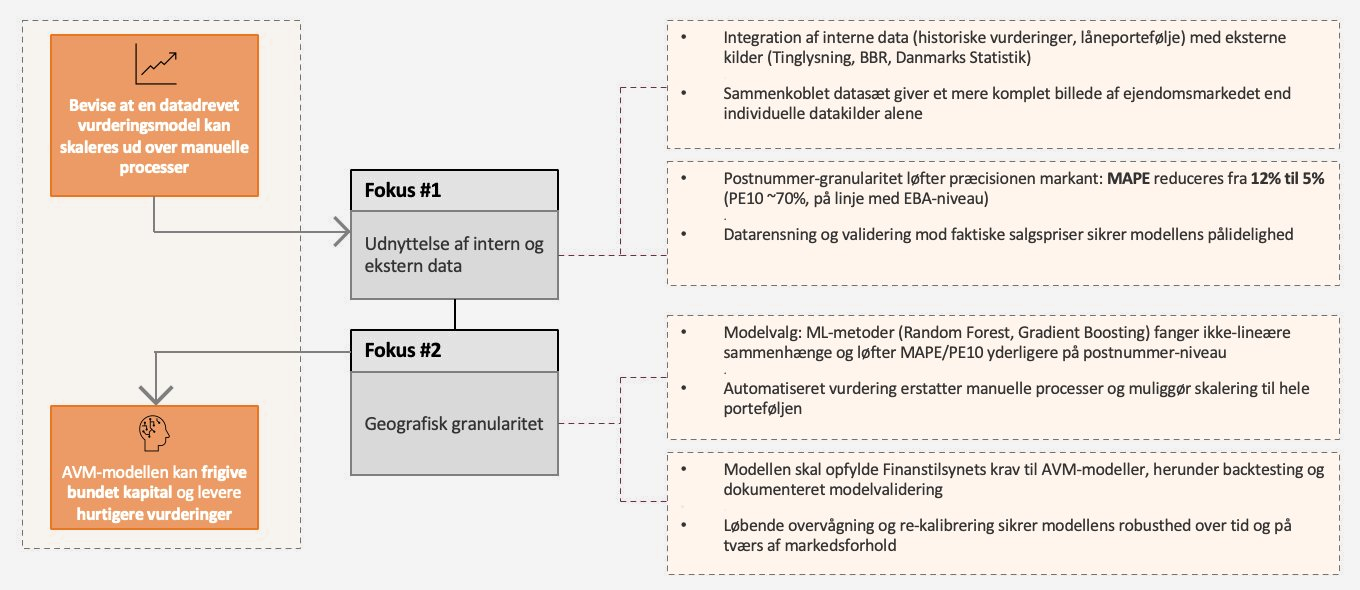
\includegraphics[width=\textwidth]{issue_tree_korrektfarve.png}
    \caption{Issue-tree for AVM-implementering hos Totalkredit. Kilde: egen visualisering.}
    \label{fig:issue_tree}
\end{figure}

\subsection{Vores strategibidrag kombinerer data og kvalitative inputs}
\label{sec:metode-bidrag}
Totalkredit er en del af Nykredit-koncernen, og denne rapport bygger på en kombination af koncernens egne, offentligt tilgængelige nøgletal, eksterne markedsdata og dialog med relevante personer i selskabets organisation. Vi anvender data fra Tinglysning.dk på historiske handelspriser og transaktioner, fra BBR på bygnings- og boligdata, og fra Danmarks Statistik på makroøkonomiske indikatorer som indkomst, befolkningsudvikling og renteniveau. Dette eksterne grundlag suppleres med intern data fra Totalkredit på porteføljens sammensætning, historiske vurderinger og operationelle omkostninger ved vurderingsprocessen. Tilsammen leverer disse kilder et kvantitativt fundament, der gør det muligt at vurdere både modellens forventede præcision og dens finansielle implikationer.

Det vigtigste kvalitative input er dialogen med Totalkredits organisation. Gennem interview med Chief Strategy Officer og dialog med vurderings- og risikofunktionerne har vi fået indsigt i, hvordan selskabet i dag prioriterer mellem manuel ekspertvurdering og automatiserede metoder, hvilke regulatoriske krav der er bindende, og hvor de største kapacitetsproblemer i den nuværende vurderingsproces opstår. Disse samtaler har været afgørende for at forstå hvilke modelfejl der i praksis er omkostningstunge, hvor langt automatisering allerede er nået internt, og hvilke konkrete forhindringer en bredere udrulning ville møde i samspillet med Finanstilsynet.

Vores bidrag er at omsætte disse inputs til en fokuseret implementeringsstrategi og en kvantificeret vurdering af dens finansielle effekt. Først identificerer vi de tre fokusområder (dataintegration, geografisk granularitet og regulatorisk governance), der tilsammen leverer det største løft i modelpræcision og operationel skalerbarhed. Dernæst kombinerer vi markedsdata og benchmarks med Totalkredits porteføljekarakteristika for at aflede et realistisk estimat af kapitalfrigivelse og omkostningsbesparelse. Strategien er udviklet uafhængigt af Totalkredit, men med løbende validering af antagelser mod de informationer, vi har fået gennem dialog med selskabet.

\begin{quote}
    \textbf{Disclaimer.} \textit{Denne rapport bygger delvist på interne estimater og offentligt tilgængelige data. Detaljerede modelparametre, prisstrukturer og specifikke porteføljedata fra Totalkredit er ikke offentliggjort af konkurrencehensyn, og enkelte tal omkring kapitalfrigivelse og besparelser er illustrative og baseret på rimelige antagelser. Hvor antagelser er kritiske for konklusionen, dokumenteres og kvantificeres følsomheden eksplicit i kapitel~\ref{sec:finans}.}
\end{quote}

\newpage

% =====================================================================
\section{Situation \textbar{} Totalkredit står stærkt, men kapitaloptimering kræver mere præcis LTV-overvågning}
\label{sec:situation}

\subsection{Totalkredit er Danmarks dominerende realkreditinstitut}
\label{sec:sit-marked}
Totalkredit har siden etableringen i 1990 udviklet sig fra et samarbejde mellem lokale og regionale pengeinstitutter til det største realkreditinstitut i Danmark målt på markedsandel inden for private boligejere \parencite{totalkredit2023}. Selskabet er i dag en helejet del af Nykredit-koncernen og distribuerer sine produkter gennem ca. 50 samarbejdende pengeinstitutter. Denne distributionsmodel betyder, at Totalkredit har adgang til et betydeligt geografisk fodaftryk uden selv at drive et filialnet, hvilket både holder de operationelle omkostninger lave og giver en bred kontaktflade til kunderne på tværs af landet.

På realkreditmarkedet for private boligejere har Totalkredit en andel på ca. 52 procent og en samlet udlånsmasse på knap 1.000 mia. kr., fordelt på mere end en million aktive lån (figur~\ref{fig:markedsandel}). Den nærmeste konkurrent, Nordea Kredit, ligger markant lavere, og det øvrige marked deles mellem Jyske Realkredit, DLR Kredit og enkelte mindre aktører. Markedet er modent og konsolideret, og konkurrencen foregår derfor i højere grad på bidragssatser, kundeoplevelse og digitalisering end på markedsadgang. Den dominerende position giver Totalkredit en strukturel fordel: størrelsen på porteføljen er forudsætningen for, at investeringer i digitalisering kan tjenes hjem på selv små marginalforbedringer pr. lån.

Som datterselskab af Nykredit-koncernen indgår Totalkredit i koncernens overordnede digitale strategi, der peger på datadrevet kreditvurdering og porteføljestyring som centrale udviklingsspor. Det betyder, at investeringen i en datadrevet ejendomsværdimodel ikke kan ses isoleret fra koncernens øvrige initiativer; tværtimod afhænger gevinstrealiseringen af tæt synergi med Nykredits eksisterende data- og IT-infrastruktur. Det er samtidig en konkurrencemæssig pointe, at Nykredit-koncernen som helhed sidder på den største mængde interne vurderings- og lånedata i det danske marked, og at denne dataposition er det reelle fortrin, en datadrevet AVM skal monetisere.

\begin{figure}[H]
    \centering
    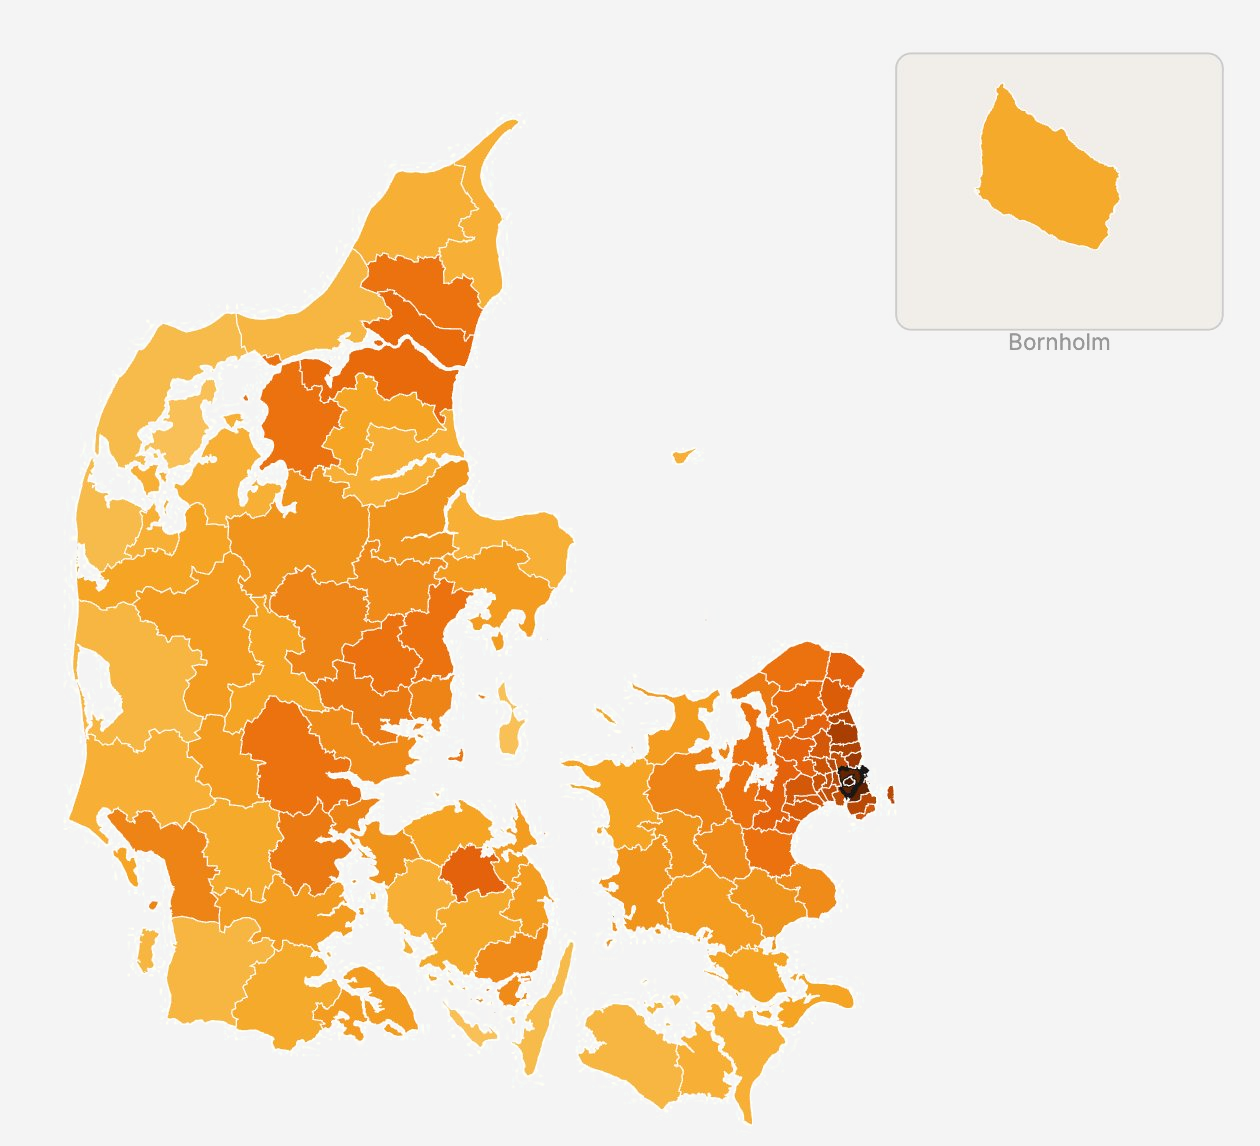
\includegraphics[width=\textwidth]{Danmarkskort_F4F4F4.png}

    \label{markedsandel}
\end{figure}
\begin{figure}[H]
    \centering
    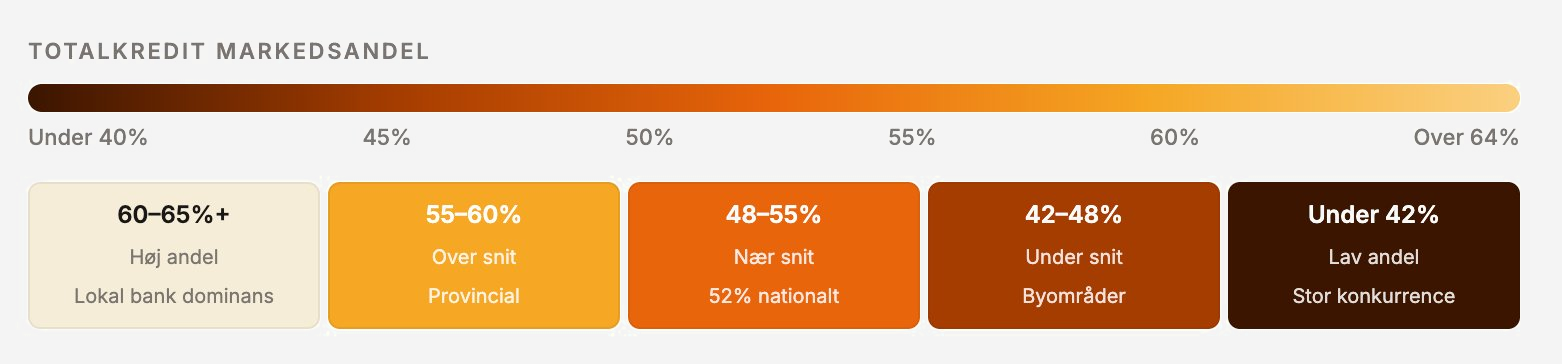
\includegraphics[width=\textwidth]{Totalkredit_legende_F4F4F4.png}
    \caption{Totalkredits markedsandel på realkreditmarkedet fordelt på danske kommuner. Kilde: Totalkredit Årsrapport 2023.}
    \label{markedsandel}
\end{figure}

\subsection{Nuværende vurderingspraksis er manuelt drevet og opdateres sjældent}
\label{sec:sit-praksis}
Den nuværende vurderingspraksis i Totalkredit er drevet af en kombination af fysiske besigtigelser udført af interne eller eksterne vurderingsspecialister, og halv-automatiske vurderinger, hvor en statistisk model giver et udgangspunkt, som en specialist efterfølgende godkender eller justerer. En typisk ejendom vurderes første gang ved låneoptagelse og opdateres derefter primært ved nye låneoptagelser, omprioriteringer eller ejerskifte. Mellem disse begivenheder opdateres den enkelte ejendoms værdi sjældent, og i en stor del af porteføljen er der i gennemsnit op til syv år mellem fysiske vurderinger.

Selskabet gennemfører i størrelsesordenen 200.000 vurderinger om året på tværs af porteføljen \parencite{totalkredit2023}. Den gennemsnitlige omkostning pr. vurdering varierer fra 3.000 til 5.000 kr. afhængigt af, om besigtigelsen er fysisk, indirekte eller alene baseret på data. Disse omkostninger er primært drevet af medarbejderløn til vurderingsspecialister, hvilket betyder, at de skalerer lineært med porteføljens størrelse og med kravet om hyppigere revurdering under CRR/CRD VI. Praksis fungerer i dag som en flaskehals: når porteføljen vokser, eller når regulatoriske krav skærper revurderingshyppigheden, må Totalkredit enten øge medarbejderstaben proportionalt eller acceptere længere intervaller mellem opdateringer.

For den enkelte ejendom betyder den lange opdateringshorisont, at den bogførte LTV-værdi systematisk afviger fra den reelle markedsværdi. En ejendom, der senest blev fysisk vurderet i 2010, vil under den nuværende model blive fremskrevet på baggrund af et bredere prisudviklingsindeks, og den faktiske afvigelse vokser jo mere prisudviklingen er afkoblet fra det lokale postnummer. Konsekvensen er en porteføljemæssig forecast error på i størrelsesordenen 10 procent, hvilket konkret afspejler sig i den buffer Totalkredit skal lægge oven på sine kapitalkrav, og i den begrænsede evne til at agere på real-time risikoeksponering.

\subsection{Tæt LTV-overvågning er forudsætning for kapitaloptimering}
\label{sec:sit-ambition}
Ejendomsværdien er det direkte input til LTV-beregningen, og LTV indgår igen i de risikovægte, der under CRR Art. 208 og CRD VI dimensionerer realkreditselskabers kapitalkrav. En lavere og bedre dokumenteret LTV udløser lavere risikovægtning og dermed lavere CET1-kapitalkrav, og det er denne mekanisme, der gør kvaliteten af ejendomsværdimodellen til et direkte finansielt parameter. På porteføljeniveau betyder forskellen mellem et forecast error på 10 procent og et forecast error på 4 procent en betydelig reduktion i den buffer, Totalkredit i dag holder for at imødegå usikkerheden i de bogførte LTV-værdier.

Finanstilsynet stiller specifikke krav til, hvornår en automatiseret vurdering må erstatte en fysisk besigtigelse. Under den nuværende model skal en ejendom typisk være fysisk besigtiget inden for tre år, før en automatiseret fremskrivning må anvendes til kreditvurderingsformål. Denne tre-års-regel binder ressourcer og forhindrer i dag Totalkredit i at udnytte sine datafortrin fuldt ud, fordi den fysiske besigtigelse i mange tilfælde reelt fungerer som en compliance-handling snarere end som en informationsskabelse. EBA's guidelines for AVM-modeller åbner for, at fuldt automatiserede vurderinger kan anvendes, hvis modellen er dokumenteret, valideret og løbende backtestet --- men det forudsætter, at Totalkredit etablerer den fornødne governance-infrastruktur.

Tre forhold gør Totalkredit til et særligt godt udgangspunkt for at investere i en datadrevet AVM. For det første har selskabet som markedsleder den største interne base af historiske vurderinger og handler, og den datamængde er fundamentet for at træne en robust vurderingsmodel. For det andet er det danske ejendomsmarked usædvanligt transparent, fordi Tinglysning.dk gør faktiske handelspriser offentligt tilgængelige, og fordi BBR leverer detaljerede bygningsdata på alle landets ejendomme. For det tredje deler Totalkredit gennem Nykredit-koncernen IT-infrastruktur og datastandarder, som reducerer de organisatoriske omkostninger ved at bygge en koncerndækkende modelplatform. Disse tre forhold tilsammen betyder, at en datadrevet AVM ikke kun er teknologisk realistisk for Totalkredit, men også at selskabet vil kunne realisere en større gevinst end konkurrenter med samme investering.

\newpage

% =====================================================================
\section{Komplikation \textbar{} Fysiske vurderinger skalerer ikke og udsætter Totalkredit for konkurrence- og regulatorisk pres}
\label{sec:komplikation}
Set isoleret kunne Totalkredit fortsætte med den nuværende vurderingspraksis. Selskabet er markedsleder, har en lønsom forretning og opfylder i dag de regulatoriske krav, der gælder for revurdering. Men praksis er omkostningstung, opdateres sjældent og efterlader et stigende gab mellem bogført og reel LTV, og dette gab har konkrete finansielle konsekvenser, der vil vokse i takt med porteføljen og med skærpede regulatoriske krav. Ledelsens spørgsmål er derfor ikke længere \textit{om} en datadrevet model er nødvendig, men \textit{hvordan} den skal udformes og implementeres, så den både frigiver kapital, sænker omkostninger og opnår regulatorisk accept.

Omkostningssiden er det mest synlige problem. 200.000 vurderinger om året multipliceret med en gennemsnitsomkostning på 3.000--5.000 kr. svarer til årlige direkte vurderingsomkostninger i omegnen af 0,6--1,0 mia. kr., og denne omkostning skalerer lineært med porteføljens størrelse. Hver gang Nykredit-koncernens digitale strategi eller en regulatorisk opdatering hæver revurderingshyppigheden, vokser omkostningen proportionalt, og Totalkredit kan ikke imødegå denne skalering uden enten at acceptere længere intervaller eller at investere i automatisering. Den manuelle proces er desuden en flaskehals, der gør det vanskeligt at reagere hurtigt på markedsudsving og umuliggør real-time porteføljestyring.

Kapitalsiden er det mindre synlige, men finansielt mere betydende problem. Når den gennemsnitlige forecast error i de bogførte ejendomsværdier ligger omkring 10 procent, må Totalkredit i sin interne risikostyring og under CRR/CRD-regelsættet holde en kapitalbuffer, der afspejler denne usikkerhed. En reduktion af forecast error til omkring 4 procent ville løfte præcisionen af LTV-overvågningen markant og dermed reducere både RWA og det implicitte kapitalkrav. På en portefølje af knap 1.000 mia. kr. svarer det til en kapitalfrigivelse, der i størrelsesordenen 2--4 mia. kr. kan anvendes til yderligere udlån eller udbetales som overskud, jf. den detaljerede beregning i kapitel~\ref{sec:finans}.

Konkurrencesiden skærper presset yderligere. Eksterne aktører som Boliga, Home og Estate driver allerede AVM-løsninger for forbruger- og mæglermarkedet, og selvom disse i dag ikke konkurrerer direkte med Totalkredits kreditvurdering, sætter de en standard for hvad kunderne forventer i form af gennemsigtighed og hastighed. Inden for Nykredit-koncernen investeres der desuden i datadrevne kreditvurderingsværktøjer, og hvis Totalkredit ikke selv driver udviklingen af en AVM målrettet realkredit, risikerer selskabet at miste sin position som koncernens datafaglige tyngdepunkt. Internt i Nykredit-koncernen er den strategiske risiko således ikke at miste markedsandel, men at miste ejerskab over den modeludvikling, der definerer fremtidens kreditbeslutninger.

Regulatorisk er Finanstilsynet og EBA's AVM-guidelines både en åbning og en betingelse. Reglerne tillader fuldt automatiserede vurderinger inden for veldefinerede rammer, men kræver dokumenteret model, løbende backtesting, intern validering og en proaktiv dialog med tilsynet. En investering i en AVM uden parallel investering i governance ville være tabt, fordi modellen ikke kunne anvendes regulatorisk. Det er kombinationen af de fire pres --- omkostninger, kapital, konkurrence og regulering --- som tvinger en samlet løsning frem, og som leder til det spørgsmål rapporten besvarer.

\paragraph{Det centrale spørgsmål.}
\begin{quote}
    \textit{Hvordan kan Totalkredit videreudvikle og implementere en datadrevet ejendomsværdimodel, der forbedrer præcisionen i den løbende LTV-overvågning og samtidig minimerer medarbejderomkostningerne til fysiske vurderinger?}
\end{quote}

\newpage

% =====================================================================
\section{Resolution: AVM-modellen \textbar{} Tre fokusområder frigiver kapital og reducerer omkostninger}
\label{sec:resolution}

\subsection{Overordnet anbefaling: tre fokusområder bygger hele modellen}
\label{sec:res-overblik}
Vores anbefaling er, at Totalkredit implementerer en datadrevet AVM-model, der bygger på tre fokusområder: dataintegration, geografisk granularitet og regulatorisk governance. De tre fokusområder er bevidst valgt, så de tilsammen adresserer alle fire pres, der blev identificeret i komplikationen: dataintegration leverer det datafundament der gør automatisering mulig og dermed adresserer omkostningssiden; postnummer-granularitet leverer den præcisionsforbedring der reducerer forecast error og dermed adresserer kapitalsiden; og regulatorisk governance sikrer at modellen reelt kan anvendes til kreditformål uden at falde i konkurrence- eller compliance-fælder.

Den underliggende model er en gradient boosting-model (XGBoost eller LightGBM), trænet på den kombinerede interne og eksterne datamængde og valideret out-of-sample mod faktiske handelspriser. machinelearning er ikke et selvstændigt fjerde fokusområde, men den tekniske ramme, der gør de tre fokusområder operationelle. Valget af gradient boosting frem for klassisk hedonisk OLS-regression motiveres af modelklassens evne til at fange ikke-lineære interaktioner mellem lokation, boligtype og makroindikatorer --- præcis de interaktioner som er centrale for præcision i geografisk heterogene markeder. Modelarkitekturen og valideringsstrategien beskrives nærmere i afsnit~\ref{sec:res-model}.

De tre fokusområder er afhængige og leveres som én samlet pakke. Dataintegration uden granularitet leverer en grov national model, der ikke udnytter datafortrin. Granularitet uden dataintegration mangler datatætheden til at undgå overfit i mindre postnumre. Og selv en perfekt model uden governance kan ikke godkendes regulatorisk og frigiver derfor ingen kapital. Det er derfor afgørende, at implementeringen behandler de tre fokusområder som ét projekt og at de finansielle gevinster i kapitel~\ref{sec:finans} alle er betingede af, at alle tre realiseres.

\subsection{Fokus \#1: Dataintegration kombinerer intern og ekstern data}
\label{sec:res-data}
Dataintegration er det første fokusområde og udgør modellens fundament. Totalkredits interne database leverer det vigtigste enkeltinput: historiske vurderinger, lån- og afdragsprofiler, geografisk metadata pr. ejendom og tidligere transaktioner i porteføljen. Disse datakilder dækker over en million aktive lån og udgør derfor et tilstrækkeligt grundlag til at træne en granulær forudsigelsesmodel for langt størstedelen af det danske boligmarked. Den interne datamængde er kvalitetsmæssigt unik, fordi den både indeholder vurderingstidspunkt, faktisk handelspris og strukturelle ejendomskarakteristika koblet ind på den enkelte ejendom.

Eksterne datakilder supplerer den interne base og er nødvendige for at fange markedsudviklingen mellem to vurderingstidspunkter. Tinglysning.dk er den vigtigste eksterne kilde og leverer faktiske handelspriser på alle danske ejendomshandler. BBR bidrager med detaljerede bygningsdata herunder areal, alder, anvendelse, antal etager og isolering. Danmarks Statistik leverer makroøkonomiske kontrolvariable som rente, befolkningsudvikling og indkomstniveau pr. kommune. DinGeo og kommercielle GIS-leverandører bidrager med afstandsdata til skoler, transport, vand og indkøb. Kombinationen af interne og eksterne kilder skaber et sammenkoblet datasæt, der dækker både den enkelte ejendoms struktur og dens markedskontekst, og som ingen enkeltkilde alene kan levere.

Den integrerede datapipeline muliggør automatisering af op mod 70 procent af de nuværende vurderinger og en reduktion af det manuelle arbejde på 50--70 procent. Konkret betyder det, at modellen leverer en automatisk vurdering, som kun eskaleres til en vurderingsspecialist, hvis modellens egen usikkerhedsestimering overstiger en defineret tærskel. Tinglysning.dk anvendes desuden løbende til at backteste modellen, fordi nye registrerede handelspriser leverer den \textit{ground truth}, der gør det muligt at måle MAPE og PE10 i realtid. Figur 3 opsummerer den samlede datakildeoversigt.

\begin{figure}[H]
    \centering
    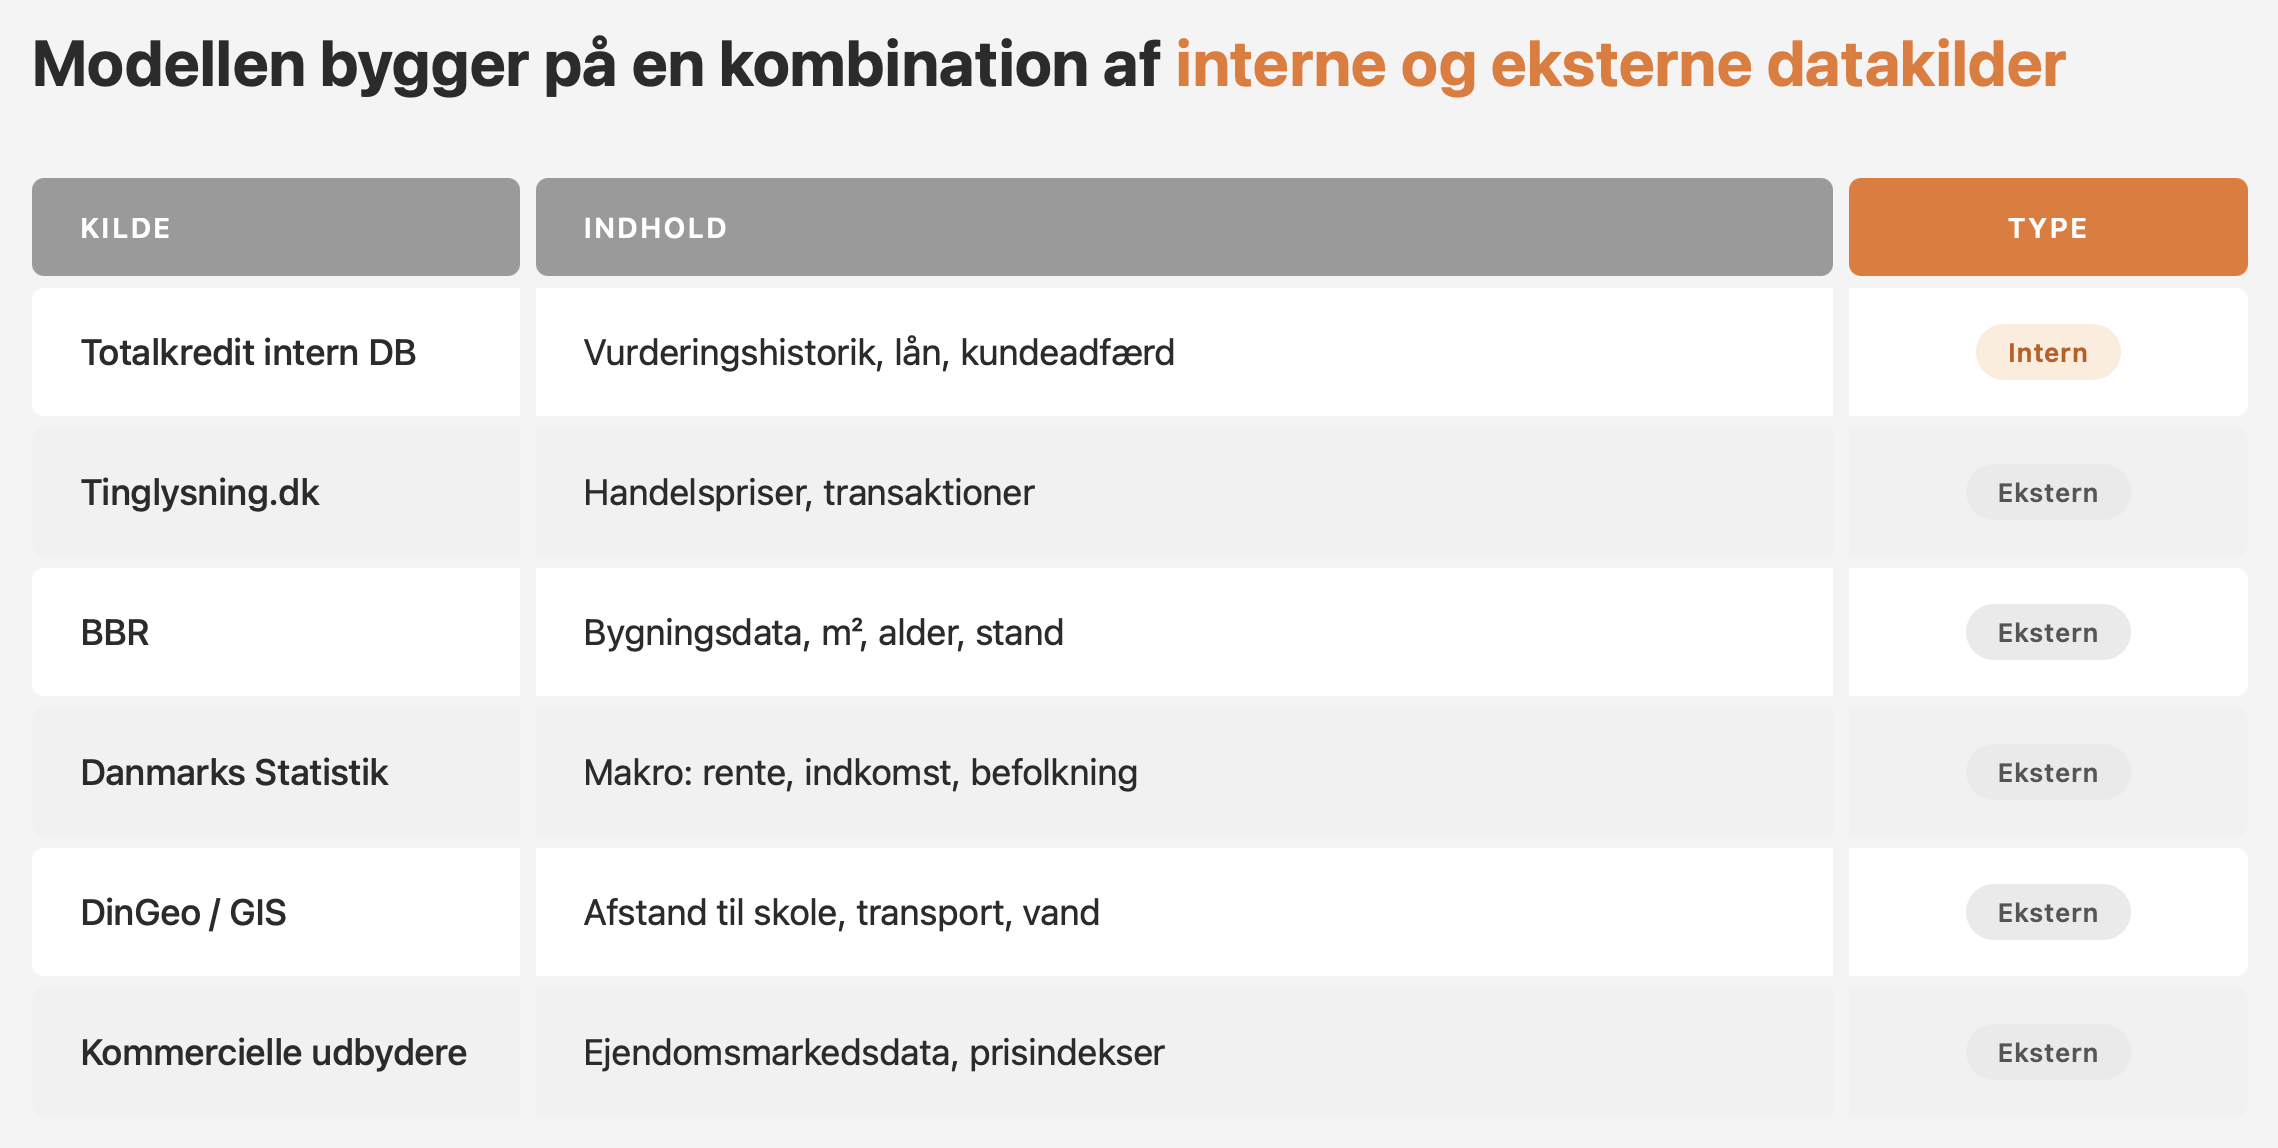
\includegraphics[width=\textwidth]{table1.png}
    \caption{Datakilder anvendt i AVM-modellen.}
    \label{data}
\end{figure}


\subsection{Fokus \#2: Geografisk granularitet på postnummerniveau}
\label{sec:res-granularitet}
Geografisk granularitet er den enkeltfaktor, der mest forbedrer modellens præcision. Boligmarkedet er fundamentalt lokalt: prisniveauet i samme bygningstype kan variere med en faktor to mellem et postnummer i indre København og et postnummer i det sydlige Sjælland, og national- eller regionalmodeller fanger ikke denne variation. Vi har derfor benchmarket modellens forventede præcision på fem geografiske niveauer (nationalt, regionalt, kommune, postnummer og kvarter), og vi finder, at postnummerniveau er den optimale balance mellem præcision og datatæthed.

Som primært performance-mål anvender vi \textit{Mean Absolute Percentage Error} (MAPE) og \textit{Percentage Error within 10\%} (PE10). MAPE udtrykker den gennemsnitlige procentvise afvigelse mellem modelvurdering og faktisk salgspris og er det mål EBA's AVM-guidelines opererer med; PE10 udtrykker hvor stor en andel af modellens vurderinger der ligger inden for $\pm$10 procent af salgsprisen og er det mål, EBA bruger til at klassificere AVM-kvalitet. En god AVM på det europæiske boligmarked har typisk en MAPE på 5--10 procent og en PE10 på 60--75 procent \parencite{ebaAVM}. Vi rapporterer R\textsuperscript{2} kun som et supplerende mål, fordi R\textsuperscript{2} mekanisk stiger med antallet af forklarende variable og derfor ikke er et pålideligt mål for prædiktiv kvalitet på usete ejendomme.

Tabel~\ref{tab:granularitet} sammenfatter den forventede modelpræcision på de fem niveauer. På postnummerniveau falder MAPE fra omkring 10 procent på det nationale niveau til omkring 4 procent, og PE10 bringes ind i det interval, EBA klassificerer som en god AVM. På kvartersniveau ses en marginal yderligere forbedring, men i over halvdelen af de danske kvarterer er antallet af årlige handler så lavt, at modellen overfit til enkelte transaktioner og dermed bliver ustabil over tid. Postnummerniveauet rammer derfor det punkt, hvor præcisionen er optimeret uden at modellen kompromitteres af dataknaphed.


\begin{figure}[H]
    \centering
    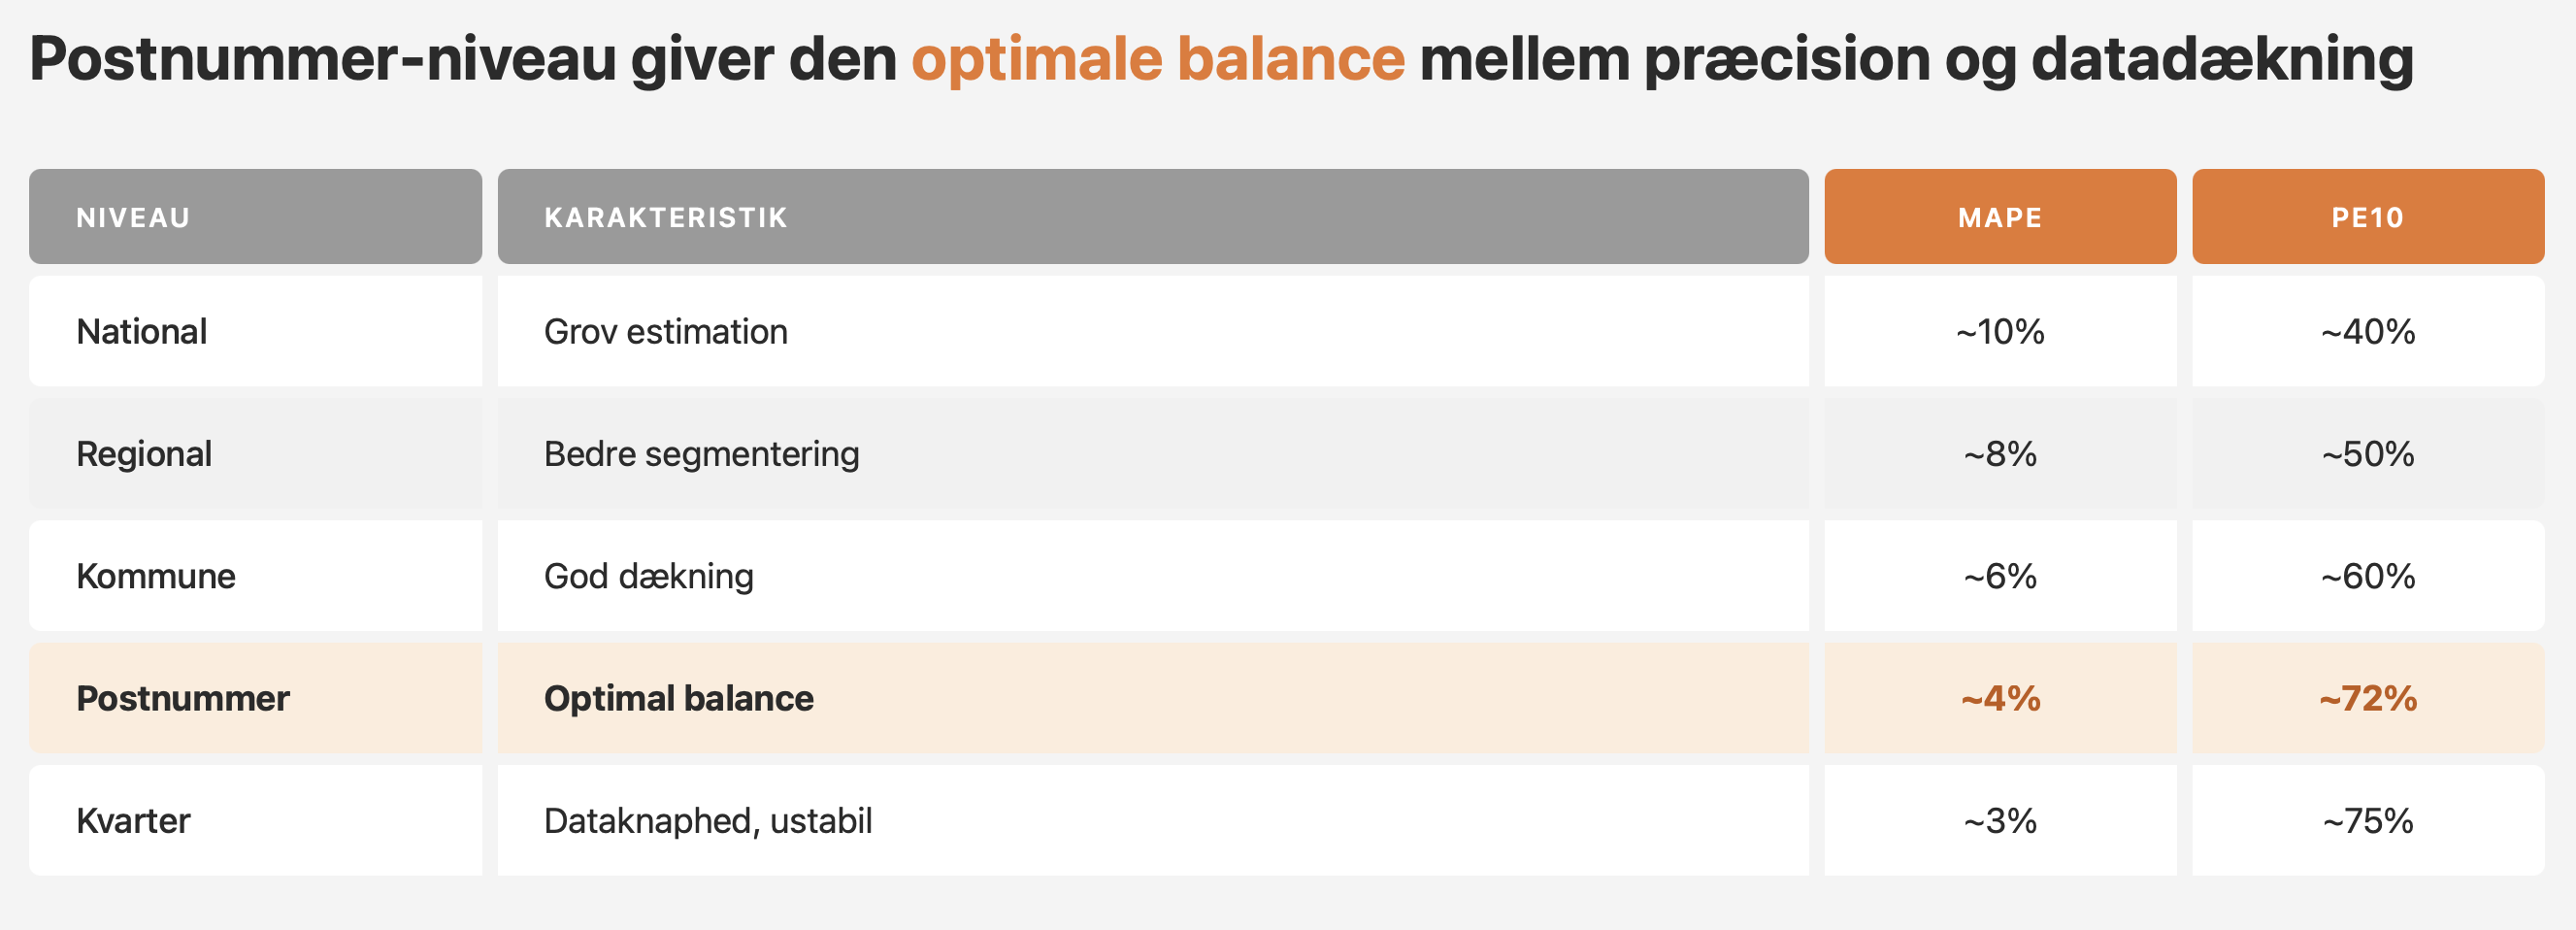
\includegraphics[width=\textwidth]{table2.png}
    \caption{Forventet modelpræcision ved forskellig geografisk granularitet.}
    \label{precision}
\end{figure}


\subsubsection{Modelvalg: gradient boosting frem for klassisk hedonisk regression}
\label{sec:res-model}
Vi anbefaler gradient boosting (konkret XGBoost eller LightGBM) som den primære modelarkitektur, kombineret med en hedonisk OLS-regression som baseline til validerings- og forklaringsformål. Gradient boosting er valgt, fordi modelklassen håndterer ikke-lineære interaktioner mellem mange forklarende variable bedre end klassisk regression, og fordi den i den internationale AVM-litteratur konsistent leverer den laveste out-of-sample MAPE på sammenlignelige boligmarkeder \parencite{mayer2019}. Modellen trænes med separate hyperparametre pr. region for at kompensere for forskelle i markedstæthed, og den anvender en en asymmetrisk tabsfunktion for samtidig at producere et punktestimat og et usikkerhedsbånd.

Validering sker via en \textit{rolling-window}-krydsvalidering, hvor modellen trænes på data frem til år $t-1$ og testes på handler i år $t$. Denne tilgang efterligner den reelle anvendelsessituation, hvor modellen ved en hvilken som helst dato kun kender historiske handler, og den undgår look-ahead bias, der ville opstå ved klassisk \textit{k-fold}-krydsvalidering på tidsseriedata. Modellen scores på MAPE og PE10 på det udeholdte år og på en stratificeret stikprøve af postnumre for at sikre, at præcisionen er ensartet på tværs af landet og ikke kun drevet af tæt befolkede områder.

Modellen leveres med en intern usikkerhedsestimering pr. ejendom, der afgør hvornår en automatisk vurdering kan accepteres, og hvornår sagen skal eskaleres til en vurderingsspecialist. Denne to-trinsproces er afgørende for den regulatoriske accept: Finanstilsynet og EBA accepterer fuldt automatiserede vurderinger inden for definerede usikkerhedsgrænser, men kræver en tydelig eskaleringsregel for vurderinger uden for grænsen. Den interne usikkerhedsestimering er derfor både et modelfagligt og et compliance-element, der bygger bro mellem fokus \#2 og fokus \#3.

\subsubsection{Forventede præcisionstab i to segmenter}
\label{sec:res-svageomr}
Selv den bedst trænede AVM vil have segmenter, hvor præcisionen er strukturelt lavere, og det er afgørende, at modellen er åben om disse begrænsninger. Vi identificerer to segmenter, hvor præcisionstabet er størst og hvor en målrettet håndtering er nødvendig.

I store vækstområder som indre København og Aarhus C kan priserne variere markant fra gade til gade, og selv et postnummer dækker over heterogene mikro-lokationer. Modellen fanger den overordnede områdetrend, men mikro-lokationsvariationen er svær at prissætte uden meget granulære features omkring eksempelvis udsigt, hjørnegrund, etage og bygningens tilstand. Vi anbefaler derfor, at modellen i disse områder suppleres med en lokal ekspertvurdering for atypiske ejendomme, samt at GIS-features bygges ud med høj opløsning på de gader, hvor mikro-variationen er størst.

I små kommuner med få årlige handler er problemet det modsatte. Datatætheden er for lav til at modellen kan lære kommunespecifikke prismønstre robust, og enkelte atypiske huse kan skævvride vurderingen for hele kommunen. For disse segmenter anvender vi en \textit{Bayesian shrinkage}-mekanisme, der vægter modelvurderingen mod det regionale gennemsnit i takt med, at den lokale datatæthed falder. Dette giver en mere konservativ vurdering i sparsomme områder og forhindrer at modellen tager store gambles på baggrund af få observationer, og det er samme tilgang som flere internationale AVM-leverandører anvender med succes på sammenlignelige markeder.

\subsection{Fokus \#3: Regulatorisk governance fra dag ét}
\label{sec:res-governance}
Regulatorisk governance er det tredje fokusområde og er forudsætningen for, at de finansielle gevinster i kapitel~\ref{sec:finans} reelt kan realiseres. En AVM, der ikke er regulatorisk godkendt, kan ikke anvendes som grundlag for kreditbeslutninger eller for LTV-rapportering, og dermed leveres hverken kapitalfrigivelsen eller omkostningsbesparelsen. Vi anbefaler derfor, at governance-arkitekturen designes ind i projektet fra dag ét og at dialogen med Finanstilsynet indledes inden modellen er færdigudviklet.

Finanstilsynets vejledning om vurderingspraksis stiller krav om en dokumenteret og forsvarlig vurderingspraksis, og om at AVM-modeller valideres og backtestes løbende \parencite{finanstilsynet2024}. Kombinationen af modelvurdering og ekspertvurdering accepteres eksplicit, hvilket understøtter den to-trinsproces vi anbefaler i afsnit~\ref{sec:res-model}. Proaktiv dialog med tilsynet anbefales tidligt i projektet, fordi tilsynet i praksis tester modellens robusthed gennem en iterativ proces, og fordi tidlige feedback-runder reducerer risikoen for sene og dyre redesigns.

Under CRR Art. 208 og det kommende CRD VI er ejendomsværdien direkte input til LTV og risikovægtning, og der er krav om revurdering mindst hvert tredje år samt mindst hvert år for lån over 3 mio. kr. EBA's AVM-guidelines åbner for fuld automatisering inden for disse rammer, men kræver dokumenteret metodebeskrivelse, periodisk intern validering og at modellen indgår i stresstestscenarier for ejendomsmarkedet. Implementeringen skal derfor levere både modeldokumentation, valideringsrapporter og en stresstestramme, der kobler modellens prædiktioner med makro-scenarier.

GDPR-dimensionen håndteres ved at modeltræning sker på pseudonymiserede data, hvor ejendomsadresse og ejer er erstattet med interne ID'er, og hvor adgang til genidentifikation er rollebaseret. Databehandleraftaler indgås med alle tredjepartsleverandører, og dataklassifikation og adgangsstyring opbygges fra dag ét som en integreret del af datapipen. Det samlede governance-framework (figur~\ref{fig:governance}) består af seks løbende processer --- modeludvikling, backtesting, intern validering, Finanstilsyn-dialog, certificering og overvågning --- der kører i en lukket cyklus og sikrer, at modellen forbliver compliant over tid.


\begin{figure}[H]
    \centering
    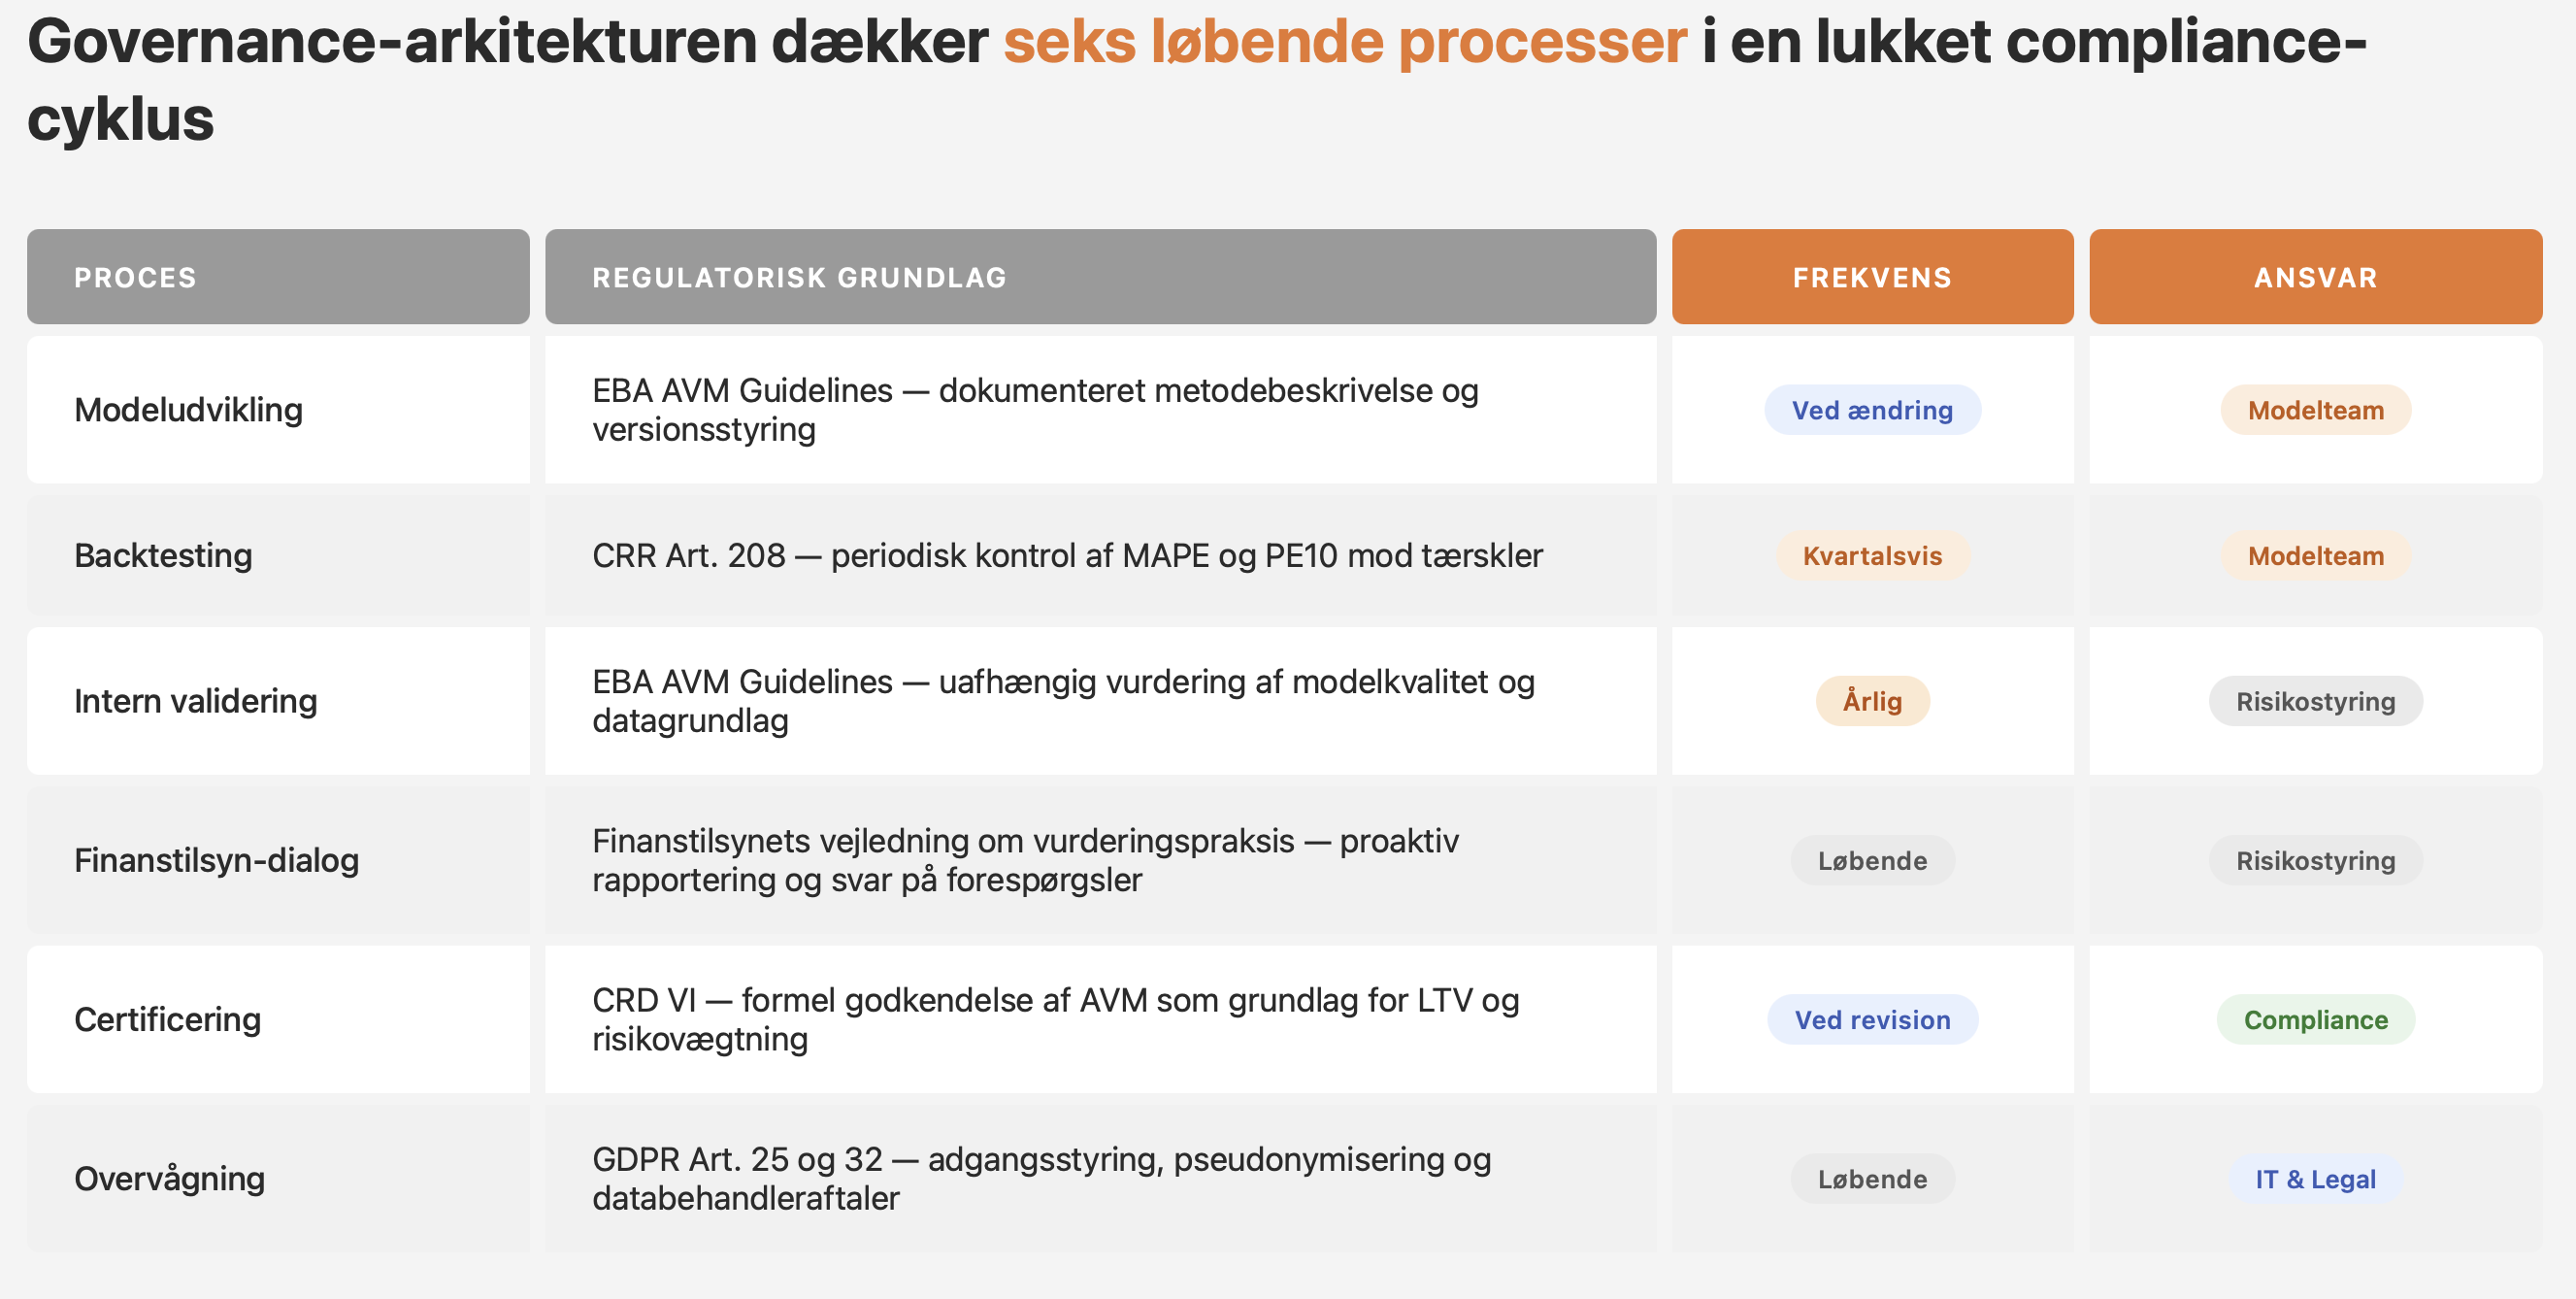
\includegraphics[width=\textwidth]{table3.png}
    \caption{Governance-loop for løbende modelvalidering og regulatorisk alignment. Kilde: egen visualisering, baseret på EBA AVM Guidelines og CRR Art.~208.}
    \label{compliance}
\end{figure}

\subsection{Benchmarking mod eksisterende AVM-løsninger}
\label{sec:res-benchmark}
AVM-modeller er ikke et nyt fænomen på det danske marked. Boliga driver en bredt anvendt forbrugervendt vurderingsmodel, der estimerer ejendomsværdier baseret på Tinglysningsdata og offentlige bygningsdata. Home og Estate driver lignende mæglervendte modeller, hvor en automatiseret prisindikation er udgangspunkt for sælgers prisforventning, og Nordea Kredit har offentligt kommunikeret, at de internt anvender en AVM som led i deres kreditvurderingsproces. Disse eksisterende løsninger sætter både en standard og et benchmark for, hvad en datadrevet AVM kan og bør levere.

Forskellen mellem Totalkredits forventede AVM og de eksisterende løsninger ligger primært i tre forhold. For det første har Totalkredit som markedsleder adgang til den største interne base af historiske vurderinger og lånedata; ingen forbruger- eller mæglervendt model har adgang til denne kombination af handelsdata og kreditdata på et halvdelen-af-markedet-niveau. For det andet er Totalkredits AVM designet til kreditformål og ikke til prismarkedsføring, hvilket betyder, at modellen optimeres for konservatisme og dokumenterbarhed snarere end for forbrugervenligt ``salgs-tagline''. For det tredje sker integrationen med kreditbeslutningen direkte, og modellen kan derfor anvendes til løbende porteføljestyring frem for kun til transaktionsbeslutninger.

Den strategiske implikation er, at Totalkredit ikke konkurrerer med Boliga og Home om forbrugerens opmærksomhed, men derimod udnytter en strukturel datafordel, som ingen ekstern aktør kan replikere. Inden for Nykredit-koncernen er Totalkredits AVM endvidere positioneret til at blive den koncerndækkende modelplatform for boligværdiansættelse, hvilket forstærker investeringscasen yderligere ved at sprede de faste udviklingsomkostninger over en større anvendelsesbase.

\newpage

% =====================================================================
\section{Finansiel implikation \textbar{} 2--4 mia. kr.\ kapitalfrigivelse og 42--70 mio. kr.\ årlige besparelser}
\label{sec:finans}
Den finansielle effekt af den anbefalede AVM-model består af to komponenter, der hver især leverer en betydelig værdi til Totalkredit. Kapitalfrigivelse er den største enkeltkomponent og er drevet af reduktionen i forecast error på de bogførte ejendomsværdier; omkostningsbesparelse er den mest direkte komponent og er drevet af den 70-procents reduktion i fysiske vurderinger, som dataintegrationen muliggør. Begge komponenter er konservativt estimeret og bygger på offentligt tilgængelige nøgletal og rimelige antagelser om Totalkredits porteføljekarakteristika.

\subsection{Sammenligning: status quo vs.\ datadrevet model}
\label{sec:fin-tabel}
Tabel~\ref{tab:statusquo} sammenfatter den samlede finansielle effekt på tværs af de centrale parametre. Antallet af fysiske vurderinger reduceres fra ca. 200.000 til ca. 60.000 om året, fordi modellen overtager vurderingen for de cirka 70 procent af porteføljen, hvor den interne usikkerhedsestimering ligger under tærsklen. Den gennemsnitlige omkostning pr. vurdering falder til omkring 800 kr. i de tilfælde, hvor modellen leverer vurderingen, da omkostningen i disse tilfælde er drevet af IT-drift snarere end medarbejdertid. Forecast error på LTV-estimaterne forbedres fra omkring 10 procent til omkring 4 procent, og PE10 bringes ind i det interval, EBA klassificerer som en god AVM.

\begin{figure}[H]
    \centering
    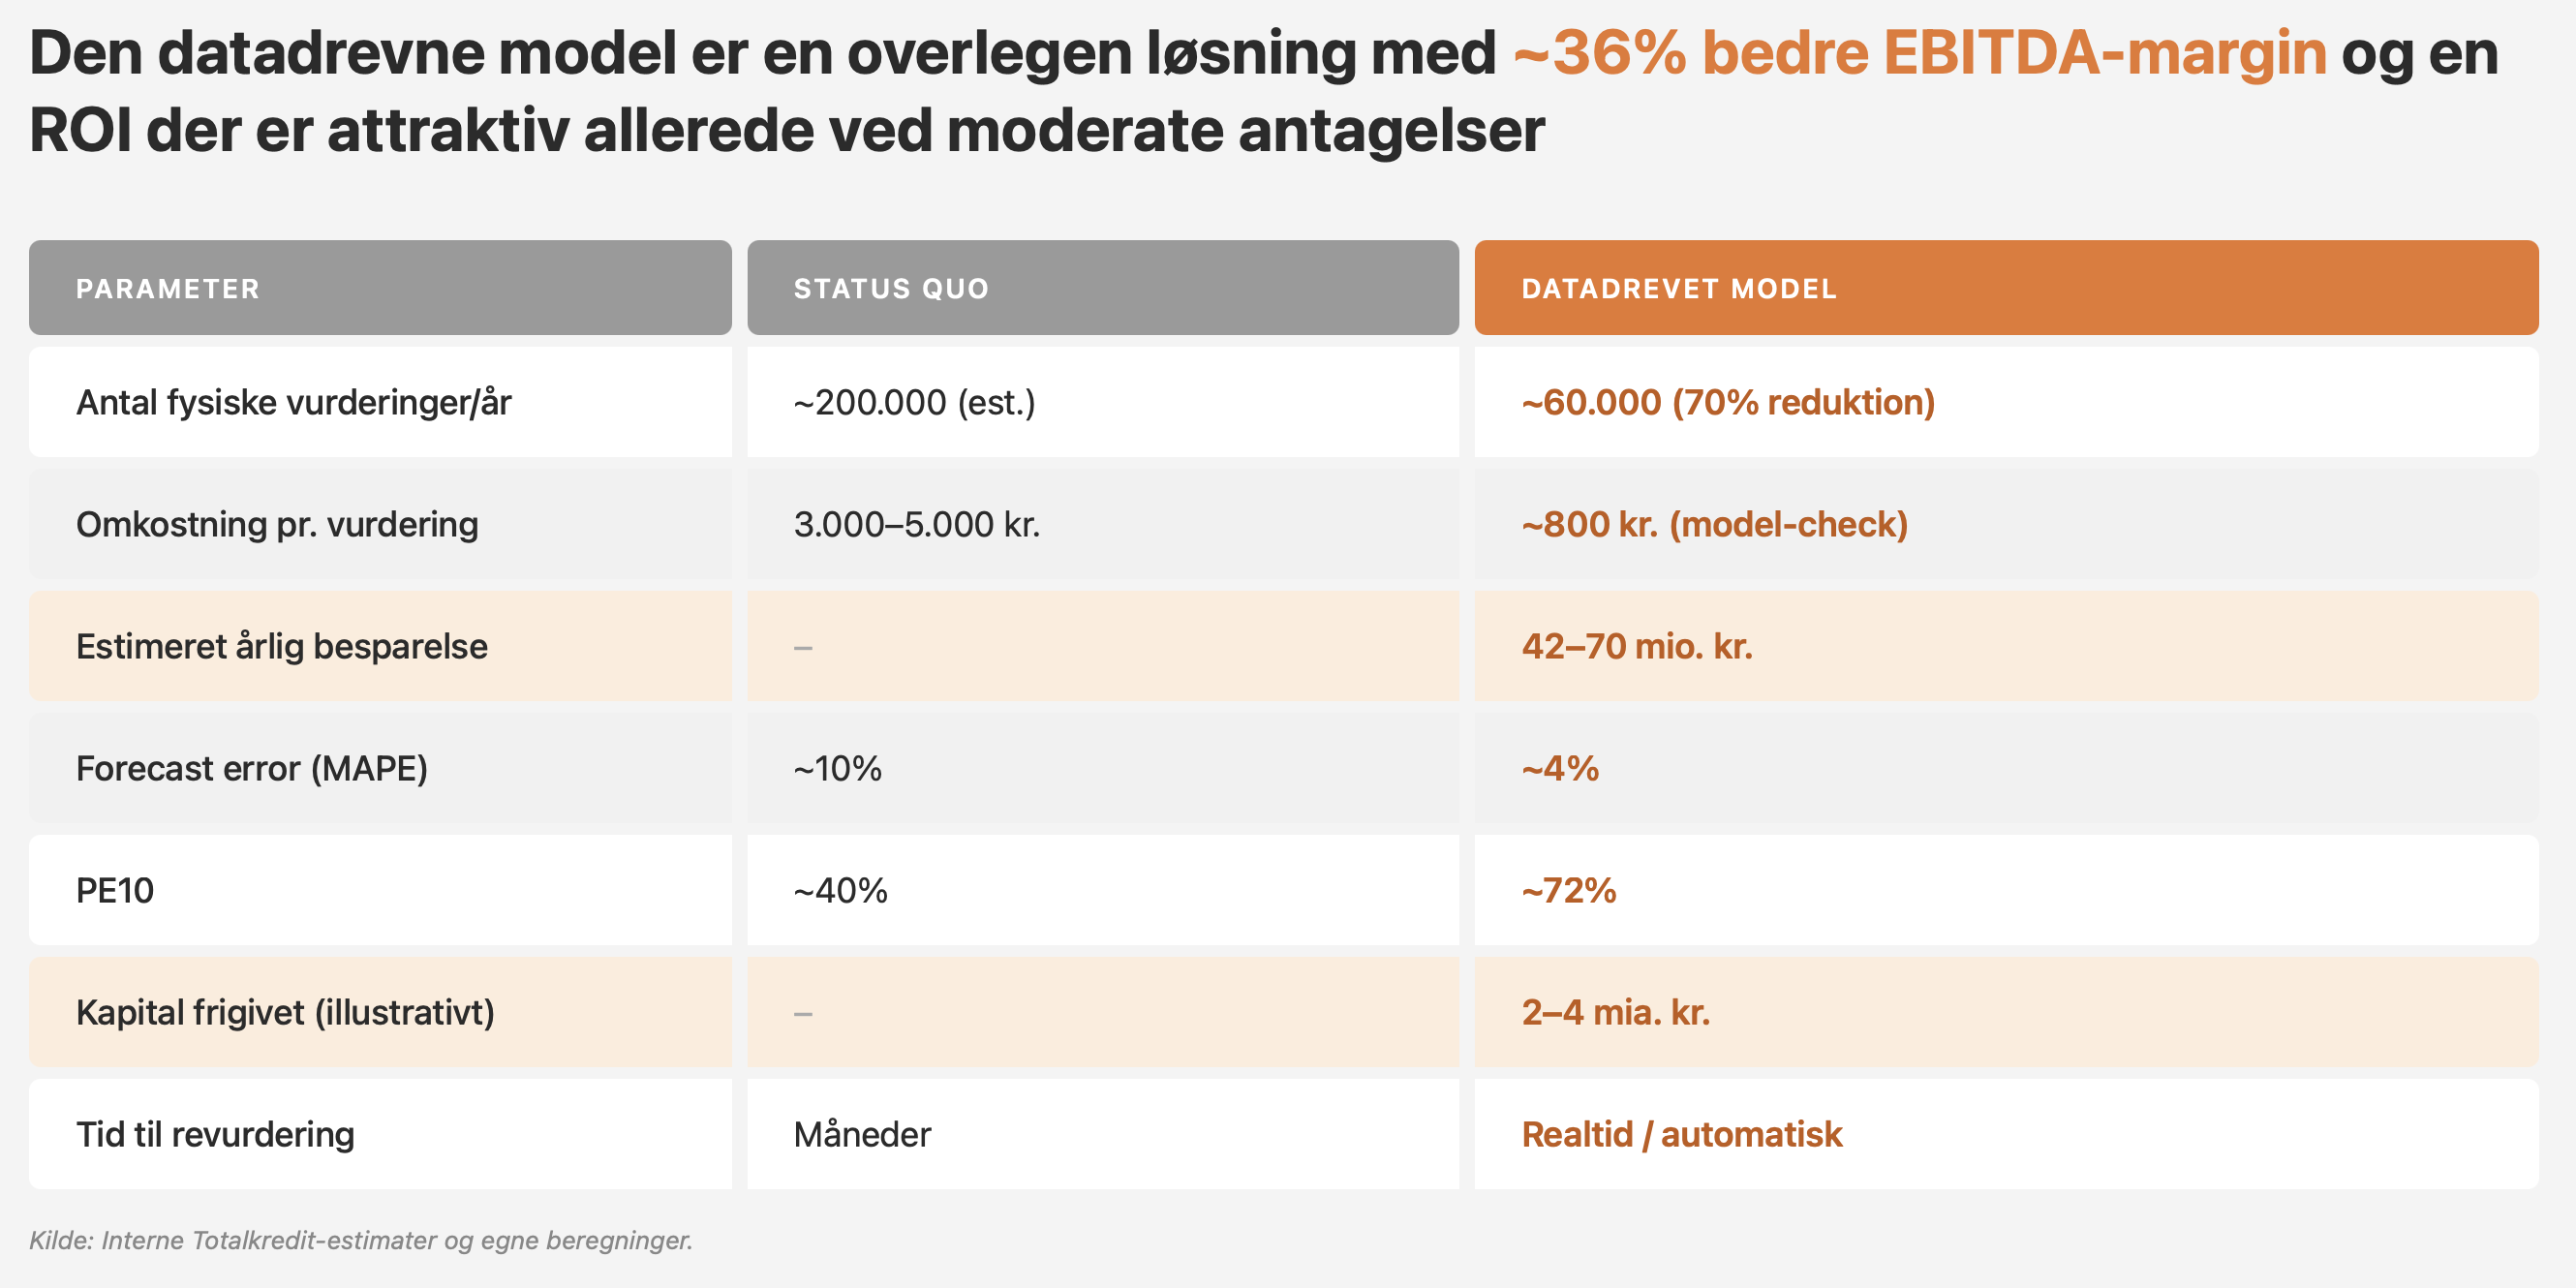
\includegraphics[width=\textwidth]{table4.png}
    \caption{Interne Totalkredit-estimater og egne beregninger.}
    \label{estimates}
\end{figure}

På tværs af komponenterne leverer den anbefalede model en strukturelt overlegen unit-økonomi sammenlignet med status quo: variable omkostninger sænkes med 50--70 procent, kapitalintensiteten falder, og responstiden går fra måneder til realtid. Disse effekter er hver for sig betydelige, men det er kombinationen --- at de leveres af én sammenhængende investering --- som gør investeringscasen særligt attraktiv.

\subsection{Kapitalfrigivelse: lavere forecast error giver lavere RWA-buffer}
\label{sec:fin-kapital}
Kapitalfrigivelsen er en direkte konsekvens af, at LTV-estimaterne bliver mere præcise. Når LTV er bestemt med mindre usikkerhed, kan Totalkredit reducere den buffer over CET1-kapitalkravet, som selskabet i dag holder for at imødegå usikkerheden i de bogførte ejendomsværdier. Den konkrete beregning er nødvendigvis illustrativ, fordi den endelige RWA-effekt afhænger af porteføljens konkrete LTV-fordeling og af det specifikke samspil med Totalkredits interne RWA-model, men størrelsesordenen kan estimeres robust ud fra offentligt tilgængelige nøgletal.

Vi estimerer kapitalfrigivelsen via følgende illustrative beregning. Den samlede portefølje er på ca. 1.000 mia. kr., og CET1-kapitalandelen er ca. 8 procent under nuværende regelsæt. LTV-justeringskoefficienten, der beskriver hvor stor en andel af en MAPE-forbedring der oversættes til RWA-reduktion, antages at være 0,5, hvilket er konservativt sammenlignet med tilsvarende sensitivitetsanalyser i danske realkreditselskaber. Med en forecast error-reduktion på 5--6 procentpoint giver det en kapitalfrigivelse på 2--4 mia. kr., afhængigt af det konkrete scenarie. Formelt:

\begin{equation}
\Delta K_{\text{frigivet}} \;=\; P \cdot \text{CET1} \cdot \alpha_{\text{LTV}} \cdot \Delta\text{MAPE}
\label{eq:kapital}
\end{equation}

hvor $P$ er den samlede portefølje, $\text{CET1}$ er kapitalandelen, $\alpha_{\text{LTV}}$ er den marginale RWA-følsomhed over for LTV-præcision, og $\Delta\text{MAPE}$ er den forventede forbedring i forecast error. Indsætter vi konservative tal ($P=1.000$ mia. kr., $\text{CET1}=8\%$, $\alpha_{\text{LTV}}=0{,}5$, $\Delta\text{MAPE}=5$ pct.point), opnås en kapitalfrigivelse i den nedre ende af intervallet (2 mia. kr.). I et mere optimistisk scenarie ($\Delta\text{MAPE}=7$ pct.point) når kapitalfrigivelsen ca. 4 mia. kr.

Denne kapitalfrigivelse kan anvendes på flere måder. Den mest direkte anvendelse er øget udlånskapacitet, hvor Totalkredit kan øge porteføljen uden at hæve sin kapitalbase; alternativt kan den frigjorte kapital udbetales som overskud eller anvendes til konkurrencedygtige bidragssatser. Uanset anvendelsen er det værd at understrege, at kapitalfrigivelsen er en strukturel og varig effekt: så længe modellen holder sin præcision, holder den frigjorte kapital sig også frigjort.

\subsection{Omkostningsbesparelse: 70\% reduktion i fysiske vurderinger}
\label{sec:fin-omk}
Omkostningsbesparelsen er den mest direkte komponent af investeringscasen og er drevet af reduktionen i fysiske vurderinger. Vi estimerer besparelsen ud fra følgende formel:

\begin{equation}
W \;=\; N \cdot (1 - Z) \cdot P_{\text{vurd}}
\label{eq:omk}
\end{equation}

hvor $N$ er antallet af årlige vurderinger, $Z$ er den procentvise reduktion via modellen, og $P_{\text{vurd}}$ er den gennemsnitlige omkostning pr. vurdering. Med $N=200.000$, $Z=70\%$ og $P_{\text{vurd}}=3.000\text{--}5.000$ kr. opnås en årlig besparelse i intervallet 42--70 mio. kr. Denne besparelse er bruttobesparelse, og fra den skal trækkes de variable omkostninger til modeldrift (estimeret 5--10 mio. kr. årligt) og de første års afskrivning på udviklingsinvesteringen.

Det er værd at bemærke at besparelsen forventes at vokse over tid. Når Totalkredit gradvist øger automationsraten fra 70 procent mod en realistisk grænse omkring 85 procent, og når Nykredit-koncernens øvrige enheder eventuelt anvender modellen som koncerndækkende platform, kan den årlige besparelse i et modent scenarie nå et niveau over 100 mio. kr. årligt. For at undgå overestimering bygger den centrale anbefaling dog konsekvent på de 42--70 mio. kr., der er realiserbare allerede ved den initiale udrulning.

\subsection{Sensitivitet og scenarier}
\label{sec:fin-sens}
For at vurdere robustheden af den finansielle gevinst har vi gennemregnet tre scenarier. I det konservative scenarie antages en lavere automatiseringsrate (50 procent), en lavere gennemsnitsomkostning pr. vurdering (3.000 kr.) og en mindre forecast error-forbedring (3 pct.point). I baseline-scenariet anvendes de centrale antagelser fra afsnit~\ref{sec:fin-kapital}--\ref{sec:fin-omk}. I det aggressive scenarie antages en højere automationsrate (85 procent), en højere gennemsnitsomkostning pr. vurdering (5.000 kr.) og en større forecast error-forbedring (7 pct.point).

\begin{figure}[H]
    \centering
    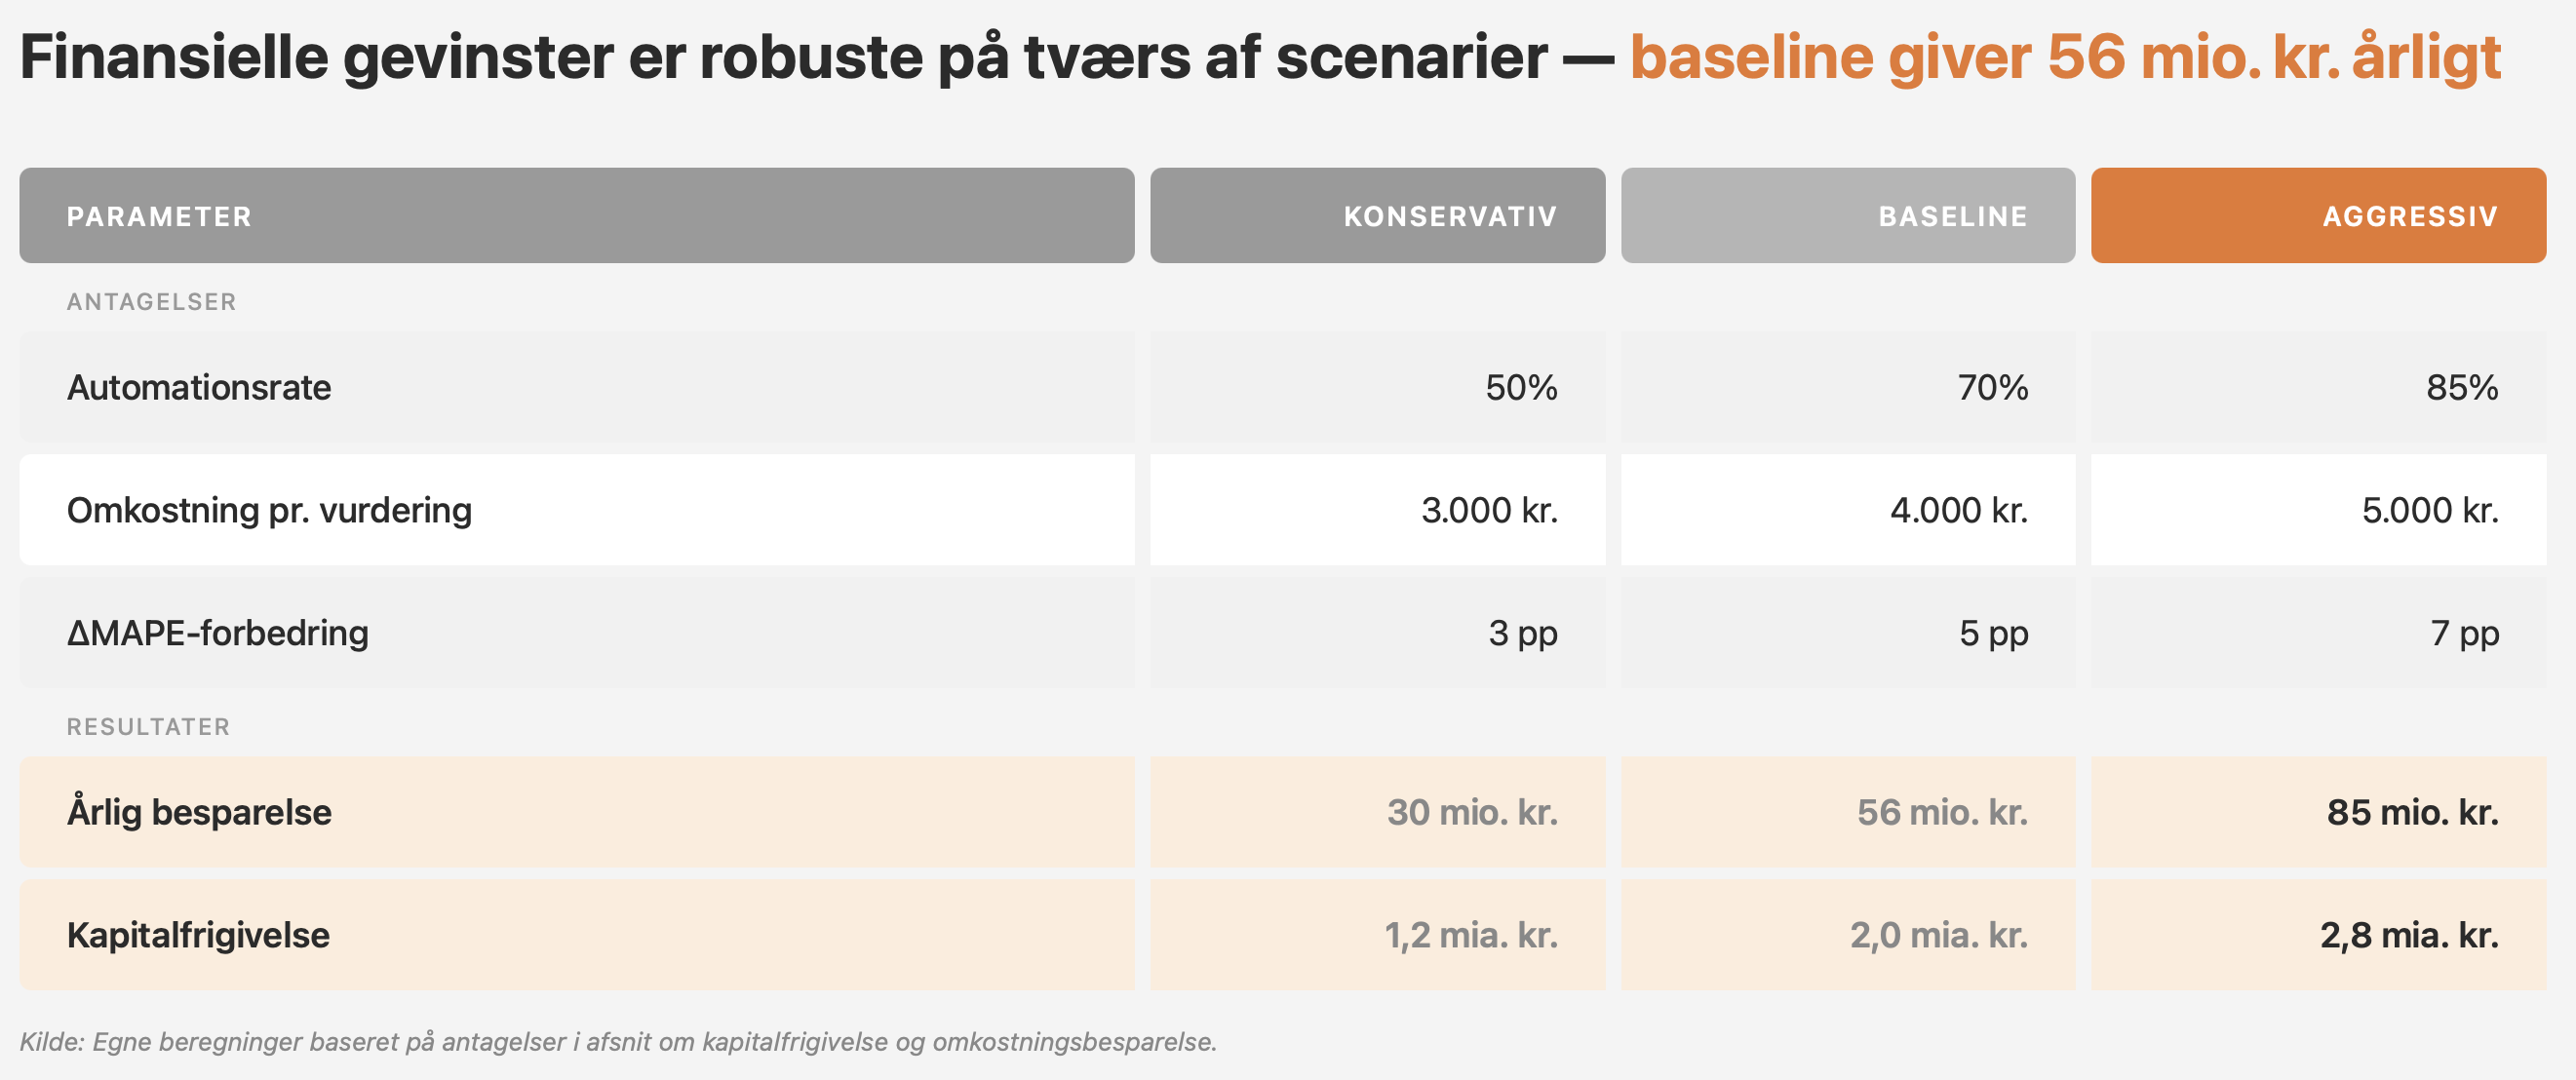
\includegraphics[width=\textwidth]{table5.png}
    \caption{Sensitivitetsanalyse: tre scenarier for finansiel effekt}
    \label{estimates}
\end{figure}


Selv i det konservative scenarie leverer modellen en samlet effekt på over 30 mio. kr. i årlig besparelse og over 1 mia. kr. i kapitalfrigivelse, hvilket overstiger investeringen i modeludvikling og -implementering flere gange. Investeringscasen er derfor robust over for de antagelser, der er mest usikre, og anbefalingen står ikke og falder med, om de mest optimistiske parametre realiseres.

\newpage

% =====================================================================
\section{Implementeringsplan \textbar{} Faseopdelt 12-måneders udrulning}
\label{sec:plan}
Vi anbefaler en faseopdelt 12-måneders implementeringsplan, der minimerer risiko og muliggør løbende regulatorisk alignment. Planen er bevidst designet til at frontloade dataarbejdet og governance-dialogen, fordi det er disse to elementer, der historisk har været årsagen til forsinkelser i lignende AVM-projekter i den finansielle sektor. Først når data, modelarkitektur og regulatorisk dialog er på plads, igangsættes en kontrolleret pilottest på et udvalgt porteføljesegment, hvilket gør det muligt at iterere på modellen før den ruller ud på fuld portefølje.

Fase 1 (måned 1--3) er dataindsamling, mapping og kvalitetssikring. Den interne database kortlægges, eksterne datakilder integreres via API-aftaler med Tinglysning, BBR og Danmarks Statistik, og datakvaliteten dokumenteres. Parallelt indledes den proaktive Finanstilsyn-dialog, så tilsynet er informeret om projektet, før modeludviklingen begynder. Fase 2 (måned 4--6) er modeludvikling og feature engineering, hvor gradient boosting-modellen trænes på det kombinerede datasæt og hvor præcisionen valideres mod historiske handler. Fase 3 (måned 7--9) er en pilottest på et udvalgt porteføljesegment, fortrinsvis et geografisk område med tilstrækkelig handelsvolumen til at modellen kan testes statistisk robust. Fase 4 (måned 10--12) er Finanstilsyn-dialog og intern certificering, hvor modellen formelt godkendes til kreditformål. Endeligt sker den fulde porteføljeudrulning og løbende overvågning fra år 2.

\begin{figure}[H]
    \centering
    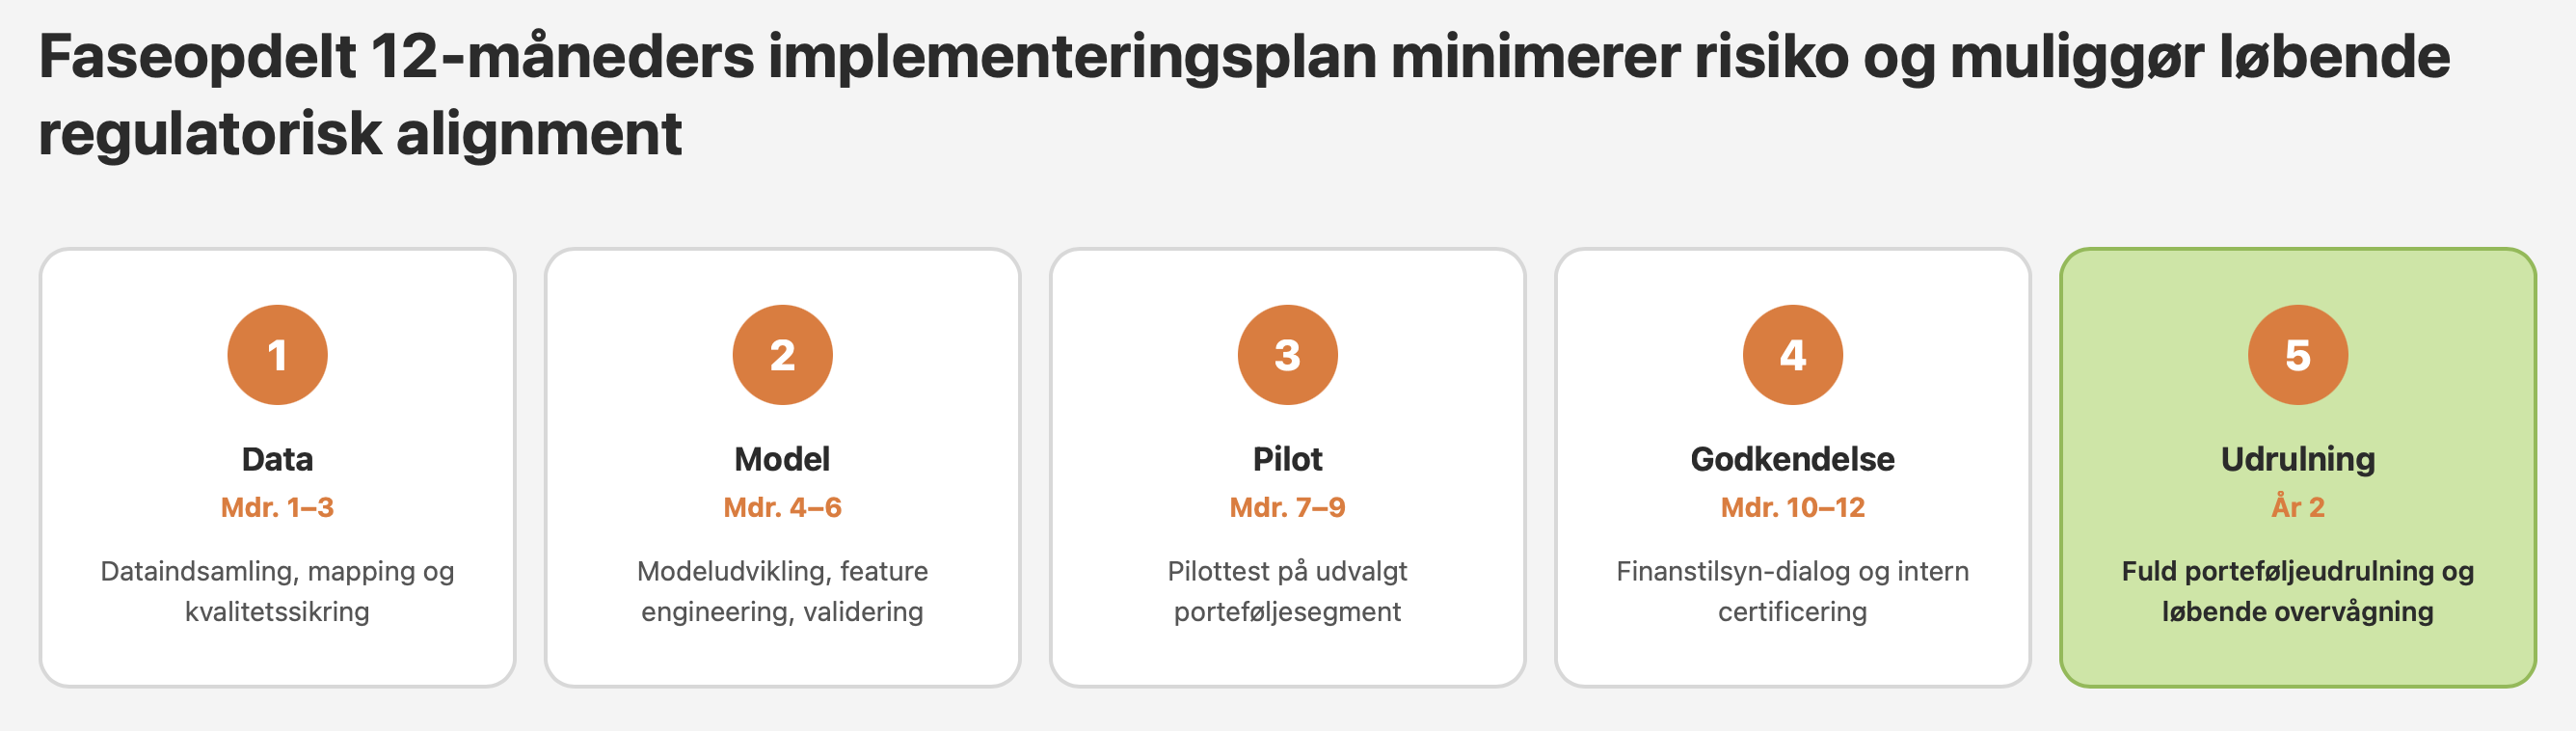
\includegraphics[width=\textwidth]{figure3.png}
    \caption{12-måneders faseplan for AVM-udrulning.}
    \label{estimates}
\end{figure}

% =====================================================================
\section{Risikovurdering}
\label{sec:risiko}
Indførelsen af en datadrevet AVM introducerer en række risici, der bør forstås, vurderes og afbødes proaktivt. De væsentligste risici er identificeret og forfinet gennem dialogen med Totalkredits Chief Strategy Officer og spænder fra datakvalitet og modelrisiko til regulatorisk forsinkelse, organisatorisk modstand og GDPR-eksponering. Tabel~\ref{tab:risiko} sammenfatter risikomatricen med sandsynlighed, konsekvens og foreslået mitigering for hver enkelt risiko.

Datakvalitet er den risiko, der vurderes som mest sandsynlig på kort sigt. Den interne database er omfattende, men ikke nødvendigvis konsistent på tværs af årtier, og dataene kan indeholde systematiske skævheder, der overføres til modellen. Vi anbefaler en systematisk kortlægning og validering i fase 1 af implementeringsplanen, hvor datakvaliteten dokumenteres og afvigelser markeres til opfølgning. Regulatorisk forsinkelse er den risiko, der har størst konsekvens, fordi en forsinket godkendelse fra Finanstilsynet udskyder hele den finansielle gevinst; risikoen mitigeres ved at indlede tilsynsdialog allerede i projektets første måned. Modelrisiko, herunder overfitting og koncept-drift over tid, mitigeres gennem out-of-sample backtesting, rolling-window krydsvalidering og periodisk intern validering, der sikrer modellens robusthed på tværs af markedsforhold.

\begin{figure}[H]
    \centering
    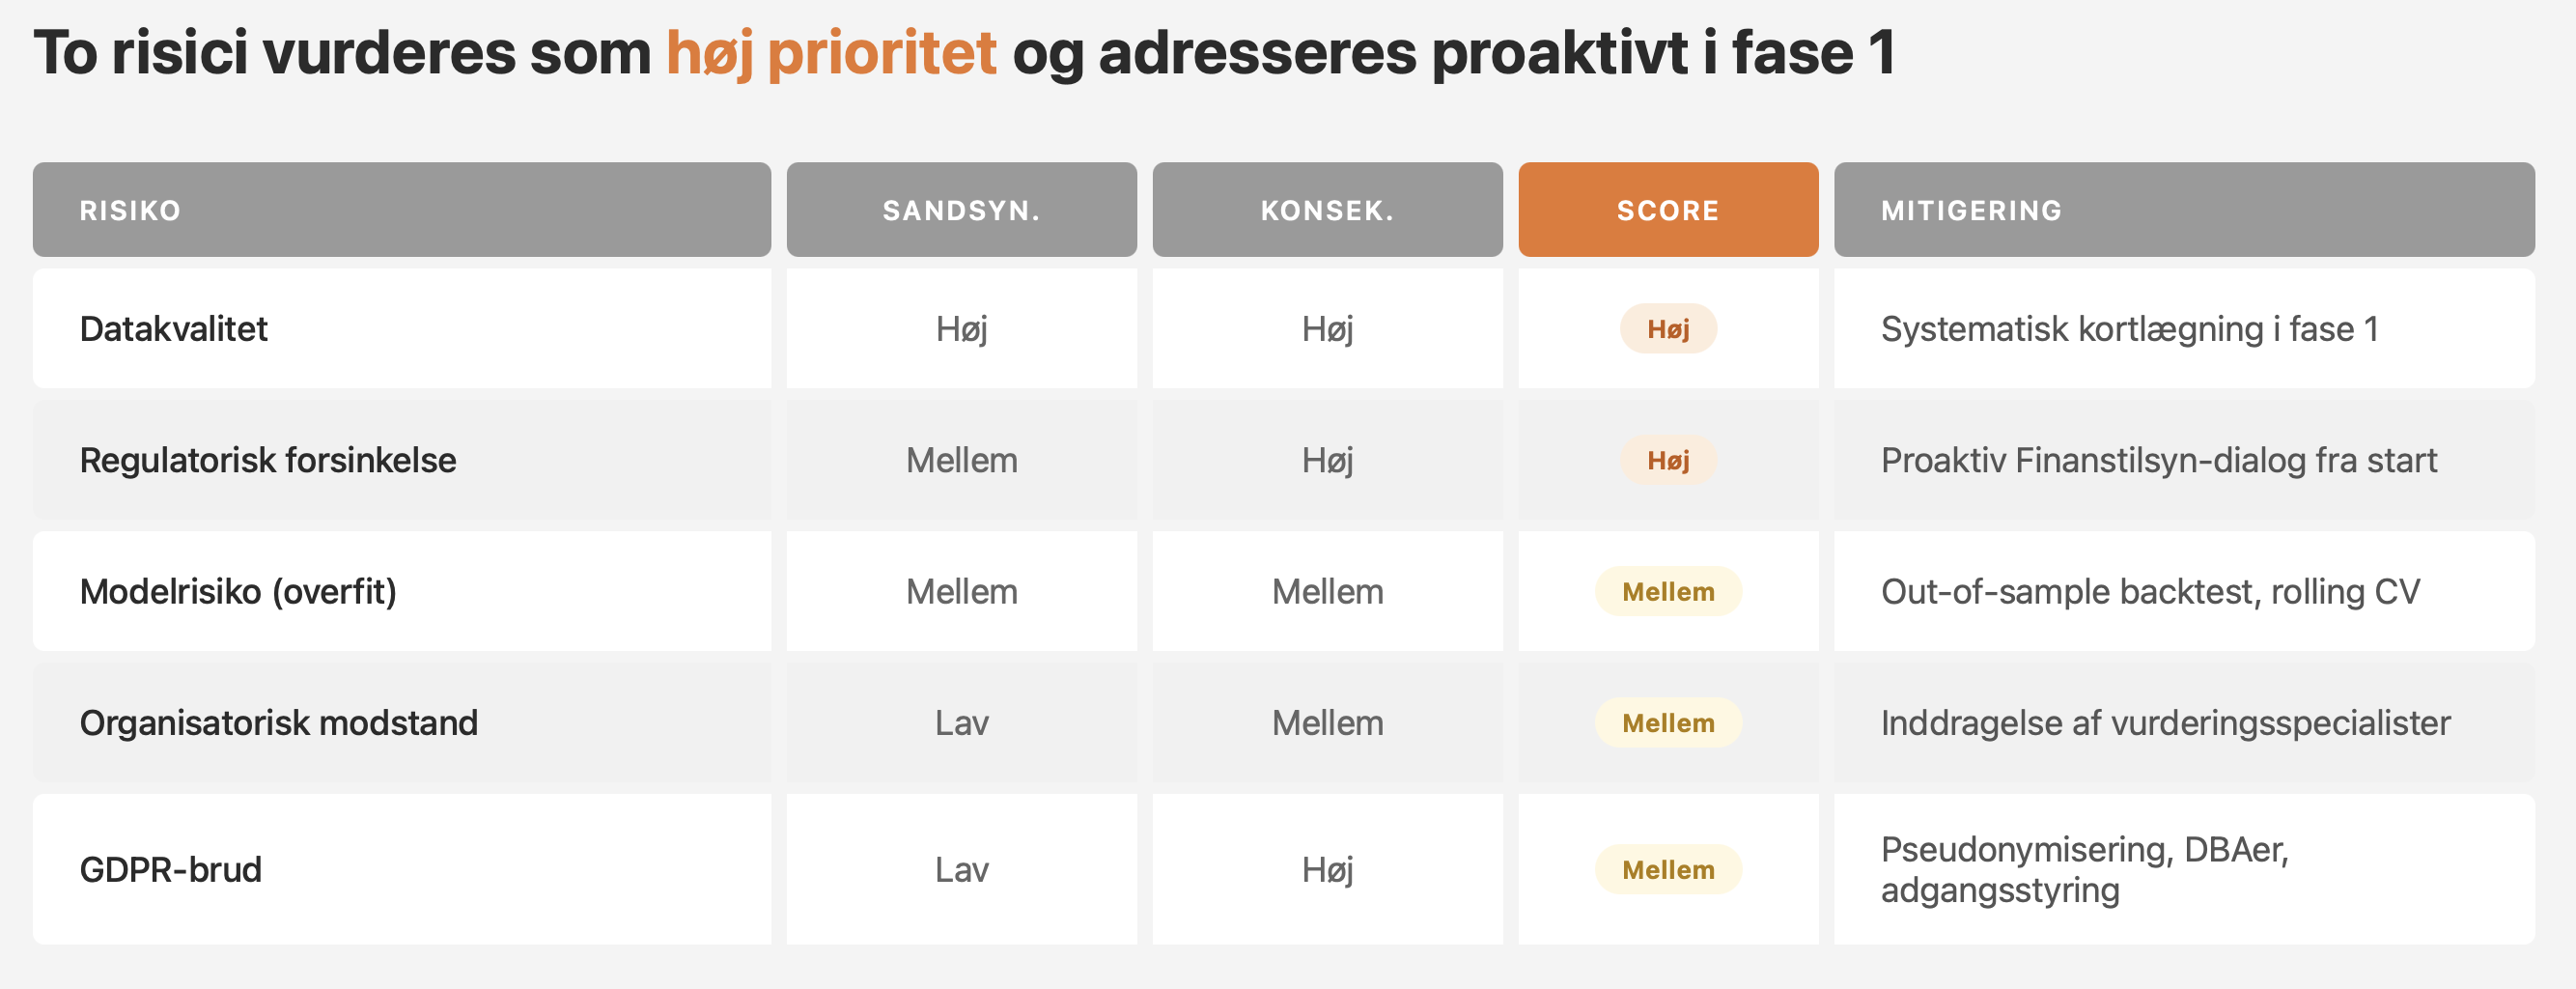
\includegraphics[width=\textwidth]{table6.png}
    \caption{Risikomatrice: sandsynlighed $\times$ konsekvens.}
    \label{estimates}
\end{figure}

\subsection{Næste skridt}
\label{sec:naeste}
Som første konkret skridt anbefaler vi, at Totalkredit i Q3 2026 etablerer et tværfunktionelt projektteam med repræsentanter fra Data, Risk og Compliance, og at projektsponsoratet placeres på direktionsniveau for at sikre tværgående beslutningskraft. Senest i samme kvartal bør den indledende dialog med Finanstilsynet finde sted, så modeludviklingen kan ske med tilsynets indledende kommentarer som rammesætning. Endeligt anbefaler vi, at beslutningen om datainfrastruktur og IT-platform træffes på koncernniveau sammen med Nykredit, så investeringen kan udnytte de eksisterende koncerndækkende systemer og samtidig positionere AVM'en som platform for fremtidig koncerndækkende anvendelse.

\newpage

% =====================================================================
\section*{Referencer}
\addcontentsline{toc}{section}{Referencer}
\printbibliography[heading=none]

\noindent\textit{Forventede referencer i den endelige rapport:}
\begin{itemize}[leftmargin=*, noitemsep]
    \item Totalkredit (2023, 2024). \textit{Årsrapport}.
    \item Nykredit (2024). \textit{Årsrapport for Nykredit-koncernen}.
    \item Finanstilsynet (2024). \textit{Vejledning om vurderingspraksis i realkreditinstitutter}.
    \item European Banking Authority (2020). \textit{Guidelines on loan origination and monitoring (EBA/GL/2020/06)} --- afsnit om AVM.
    \item Europa-Parlamentet (2013, 2024). \textit{CRR Forordning 575/2013, Art. 208; CRD VI Direktiv}.
    \item Minto, B. (2007). \textit{The Pyramid Principle: Logic in Writing and Thinking}.
    \item McKinsey \& Company (2007). \textit{The Consulting Method}.
    \item Mayer, M., Bourassa, S. C., Hoesli, M., \& Scognamiglio, D. (2019). ``Estimation and updating methods for hedonic valuation''. \textit{Journal of European Real Estate Research}.
    \item Hill, R. J. (2013). ``Hedonic price indexes for residential housing''. \textit{Journal of Economic Surveys}.
    \item Tinglysning.dk, BBR, Danmarks Statistik (datakilder).
\end{itemize}

\newpage

% =====================================================================
\section*{Appendix}
\addcontentsline{toc}{section}{Appendix}

\subsection*{Appendix A: Variabeloversigt i AVM-modellen}
Komplet feature-liste med beskrivelse, kilde og forventet effekt på ejendomsværdi. Inkluderer både kontinuerte variable (areal, alder, afstand til centrum), kategoriske variable (boligtype, anvendelse) og interaktionsvariable (postnummer $\times$ kvartalsindeks).

\subsection*{Appendix B: Robusthedstest}
Tabel med out-of-sample MAPE og PE10 pr. region pr. år (rolling window 2018--2024). Tabellen demonstrerer at modellens præcision er stabil på tværs af konjunkturcykler og at forecast error ikke systematisk er højere i specifikke regioner end andre.

\subsection*{Appendix C: Regulatorisk tjekliste}
Krydstabel der kobler hvert krav fra Finanstilsynets vejledning, CRR Art. 208, EBA AVM-guidelines og GDPR med den konkrete kontrol i modeldesignet og den ansvarlige funktion i Totalkredit.

\subsection*{Appendix D: Interviewguide}
Spørgsmål anvendt i interview med Chief Strategy Officer og dialog med vurderings- og risikofunktionerne. Interviewene er gennemført under fortrolighed, og citater er ikke gengivet direkte i rapporten.


\end{document}
